\section{Analysis}
\label{sec:analysis}


\begin{table}
\centering
\begin{tabular}{ | l | p{2.1cm} | p{1.7cm} | c |}
    \hline 
    Name & CPU & GPU & Memory \\ \hline
    \textbf{GalaxyNexus} & ARMv7, 2 cores, 1200 Mhz, SIMD NEON & PowerVR-SGX 540 & 694MB \\ \hline
    \textbf{Nexus 5} & Qualcomm Snapdragon S4 Pro 1.5GHz & Adreno 320 400MHz & 2GB \\ \hline
    \textbf{Nexus 7} & Qualcomm Snapdragon 800 2.26GHz & Adreno 330 450MHz & 2GB \\ \hline
    \textbf{Nexus 10} & DualCore 1.7GHz Cortex-A15 & Mali T604 & 2GB \\ \hline
    \textbf{SM-T900} & QuadCore 1.9GHz Cortex-A15 & Mali T628 & 3GB \\ \hline
    \hline
\end{tabular}
\caption{The device hardware specifications used for the analysis.}
\label{table:hardware}
\end{table}

This section evaluates each benchmark on five devices shown
  in Table~\ref{table:hardware}, all running Android $4.4.2$ (KitKat).
These devices capture the low, mid, and high end mobile and tablet
  devices that are currently available in the market.
Only the Nexus 5 and Nexus 7 devices can be modified to install an
  unofficial OpenCL implementation and only those two devices are fully supported
  by Trepn.
Each benchmark contains multiple implementations, which 
  are analyzed to determine trade-offs between
  processor utilization, performance, and energy usage.
We conclude the section by discussing the programability of RenderScript
  and compare it against established programming models such as:
  native C, OpenMP, and OpenCL.

\subsection{Processor Utilization}


\begin{figure*}[ht]
  \centering

  \begin{subfigure}[b]{\textwidth}
          \centering
          
\includegraphics[width=0.4\textwidth]{data/load_legend.pdf}
  \end{subfigure}

  \begin{subfigure}[b]{0.9\textwidth}
       \centering
       
\includegraphics[width=\textwidth]{data/load_vectoradd_nexus5.pdf}
       \caption{VectorAdd on Nexus 5}\label{fig:Vecadd5}
   \end{subfigure}
  \begin{subfigure}[b]{0.9\textwidth}
       \centering
       
\includegraphics[width=\textwidth]{data/load_vectoradd_nexus7.pdf}
       \caption{VectorAdd on Nexus 7}\label{fig:Vecadd7}
   \end{subfigure}

  \begin{subfigure}[b]{0.9\textwidth}
       \centering
       
\includegraphics[width=\textwidth]{data/load_sgemm_nexus5.pdf}
       \caption{Sgemm on Nexus 5}\label{fig:Sgemm5}
   \end{subfigure}
  \begin{subfigure}[b]{0.9\textwidth}
       \centering
       
\includegraphics[width=\textwidth]{data/load_sgemm_nexus7.pdf}
       \caption{Sgemm on Nexus 7}\label{fig:Sgemm7}
   \end{subfigure}


  \caption{Processor utilization of VectorAdd and SGEMM for both Nexus 5 and Nexus 7. The Y axis is normalized across implementations with $1$ representing the peek utlization ($frequency*load$) for CPUs or GPUs. The X axis encodes timed blocked and is not scaled across implementations.}
  \label{fig:loadVecAddSgemm}
\end{figure*}
\FloatBarrier

Mobile devices use dynamic voltage frequency scaling (DVFS)
  to match performance to power utlization.
The frequency is increased for the processors when the load goes over a certain
  threashold.
Both CPUs and GPUs make use of frequency scaling, but unlike CPUs (which typically
  have vary fine frequencies --- operating at around 10 different frequencies), GPUs
  have coarse grained frequencies (operating at only 4 different frequencies).  

Processor utlization is measured by multiplying the $frequency$ and the $load$ information collected via Qualcomm's Trepn~\cite{profilerqualcomm} tool.
The performance times are measured with the system connected to a
  power source, which avoids the device going to sleep (it does add the
  overhead of the device comunicating debug information with the development
  machine).
Since Trepn has a $100ms$ measure granularity, the kernel code is run $100$ times
  ($5$ times for MRIQ and TPACF), this allows us to visualize the trend in resource
  utlization.
The information gives us insight as to what parts of the code are active in each
	section of the code, how that impacts performance and battery.


Note that Java UI thread is running independent of the computation as well as Trepn which
  have a high overhead ($10\%$ on average).
These background processes are echoed in
  the plots --- a single threaded Java code, for example, should not utilize more than one core, but our plots show that more than one core is active.


VectorAdd has a very high memory to compute ratio, therefore the processor utlization
  plot~(figure \ref{fig:loadVecAddSgemm}) shows that not all CPUs 
  are fully utlized during the compute phase.
For the Nexus 5 device, while the graphs show a GPU is being used during the OpenMP,
  Renderscript, and Java, this is an error in the measurement --- we believe this is 
  due to the UI thread utilizing the GPU or some other interferences.
As expected, the GPU is not being utilized on the Nexus 7 except for OpenCL.

As discussed in the benchmark section, the Android GCC compiler was not able 
  to interpret the OpenMP pragma code and therefore SGEMM runs in a single thread
  on both the Nexus 5 and Nexus 7 (figure~\ref{fig:loadVecAddSgemm}).
While OpenCL does utlize the GPU, because of the size of the matrix, there GPU has
  lower occupancy and therefore does not achieve peek performance.
Both the RenderScript and ThreadedJava code make full utlization of all the cores.

MRIQ is embarisingly parallel and we can see full utlization for both the CPUs and GPUs in figure~\ref{fig:loadMRIQTpacf}.
Abrupt dips in the plots show positions where a kernel launch occurs.
It is also interesting to note that on the Nexus 5 the CPU is not fully utilized for both ThreadedJava and Renderscript.
This is due to either the load being low for a high frequency or the frequency being 
  choosen to be low.

\begin{figure*}[ht]
  \centering

  \begin{subfigure}[b]{\textwidth}
          \centering
          
\includegraphics[width=0.4\textwidth]{data/load_legend.pdf}
  \end{subfigure}

  \begin{subfigure}[b]{0.9\textwidth}
      \centering
      
\includegraphics[width=\textwidth]{data/load_mriq_nexus5.pdf}
      \caption{MRIQ on Nexus 5}
      \label{fig:MRIQ5}
  \end{subfigure}
  \begin{subfigure}[b]{0.9\textwidth}
      \centering
      
\includegraphics[width=\textwidth]{data/load_mriq_nexus7.pdf}
      \caption{MRIQ on Nexus 7}
      \label{fig:MRIQ7}
  \end{subfigure}

  \begin{subfigure}[b]{0.9\textwidth}
      \centering
      
\includegraphics[width=\textwidth]{data/load_tpacf_nexus5.pdf}
      \caption{TPACF on Nexus 5}
      \label{fig:TPACF5}
  \end{subfigure}
  \begin{subfigure}[b]{0.9\textwidth}
      \centering
      
\includegraphics[width=\textwidth]{data/load_tpacf_nexus7.pdf}
      \caption{TPACF on Nexus 7}
      \label{fig:TPACF7}
  \end{subfigure}

  \caption{Processor utilization of MRIQ and TPACF for both Nexus 5 and Nexus 7. The Y axis is normalized across implementations with $1$ representing the peek utlization ($frequency*load$) for CPUs or GPUs. The X axis encodes timed blocked and is not scaled across implementations.}
  \label{fig:loadMRIQTpacf}
\end{figure*}
\FloatBarrier

The TPACF compute codes is divided into two parts.
The first is serial computation that, for the sake of code reuse, is done on the 
  Java side using a single thread.
Once that complets, we then execute the code on different datasets in parallel.
The utlization plots (figure~\ref{fig:loadMRIQTpacf}) show this behavior.  

For Histogram (figure~\ref{fig:loadHistogramStencil}) we see that memory starts
  to play a major role in processor utlization.
The GPU is being utlized in the memory copy as it is in the computation, for example.

For Stencil (figure~\ref{fig:loadHistogramStencil}) we see that RenderScript does
  not fully utilize all CPU cores.
This is because the stencil kernel is memory access bound, performing around 10 flops 
  (ignoring index calculations).
We again see that memory copy (\fix{SetupArgs} for RenderScript and
  \fix{CopyTo} for OpenCL) result in the a substantial amound of resources being
  wasted.

\begin{figure*}[ht]
  \centering

  \begin{subfigure}[b]{\textwidth}
          \centering
          
\includegraphics[width=0.4\textwidth]{data/load_legend.pdf}
  \end{subfigure}

  \begin{subfigure}[b]{0.9\textwidth}
      \centering
      
\includegraphics[width=\textwidth]{data/load_histogram_nexus5.pdf}
      \caption{Histogram on Nexus 5}
      \label{fig:Histogram5}
  \end{subfigure}
  \begin{subfigure}[b]{0.9\textwidth}
      \centering
      
\includegraphics[width=\textwidth]{data/load_stencil_nexus5.pdf}
      \caption{Stencil on Nexus 5}
      \label{fig:Stencil5}
  \end{subfigure}

  \caption{Processor utilization of Histogram and Stencil for Nexus 5. The Y axis is normalized across implementations with $1$ representing the peek utlization ($frequency*load$) for CPUs or GPUs. The X axis encodes timed blocked and is not scaled across implementations.}
  \label{fig:loadHistogramStencil}
\end{figure*}
\FloatBarrier

\subsection{Performance}

\begin{figure*}
  \centering
  \begin{subfigure}[b]{\textwidth}
          \centering
          
\includegraphics[width=0.4\textwidth]{data/legend.pdf}
  \end{subfigure}

  \begin{subfigure}[b]{0.33\textwidth}
      \centering
      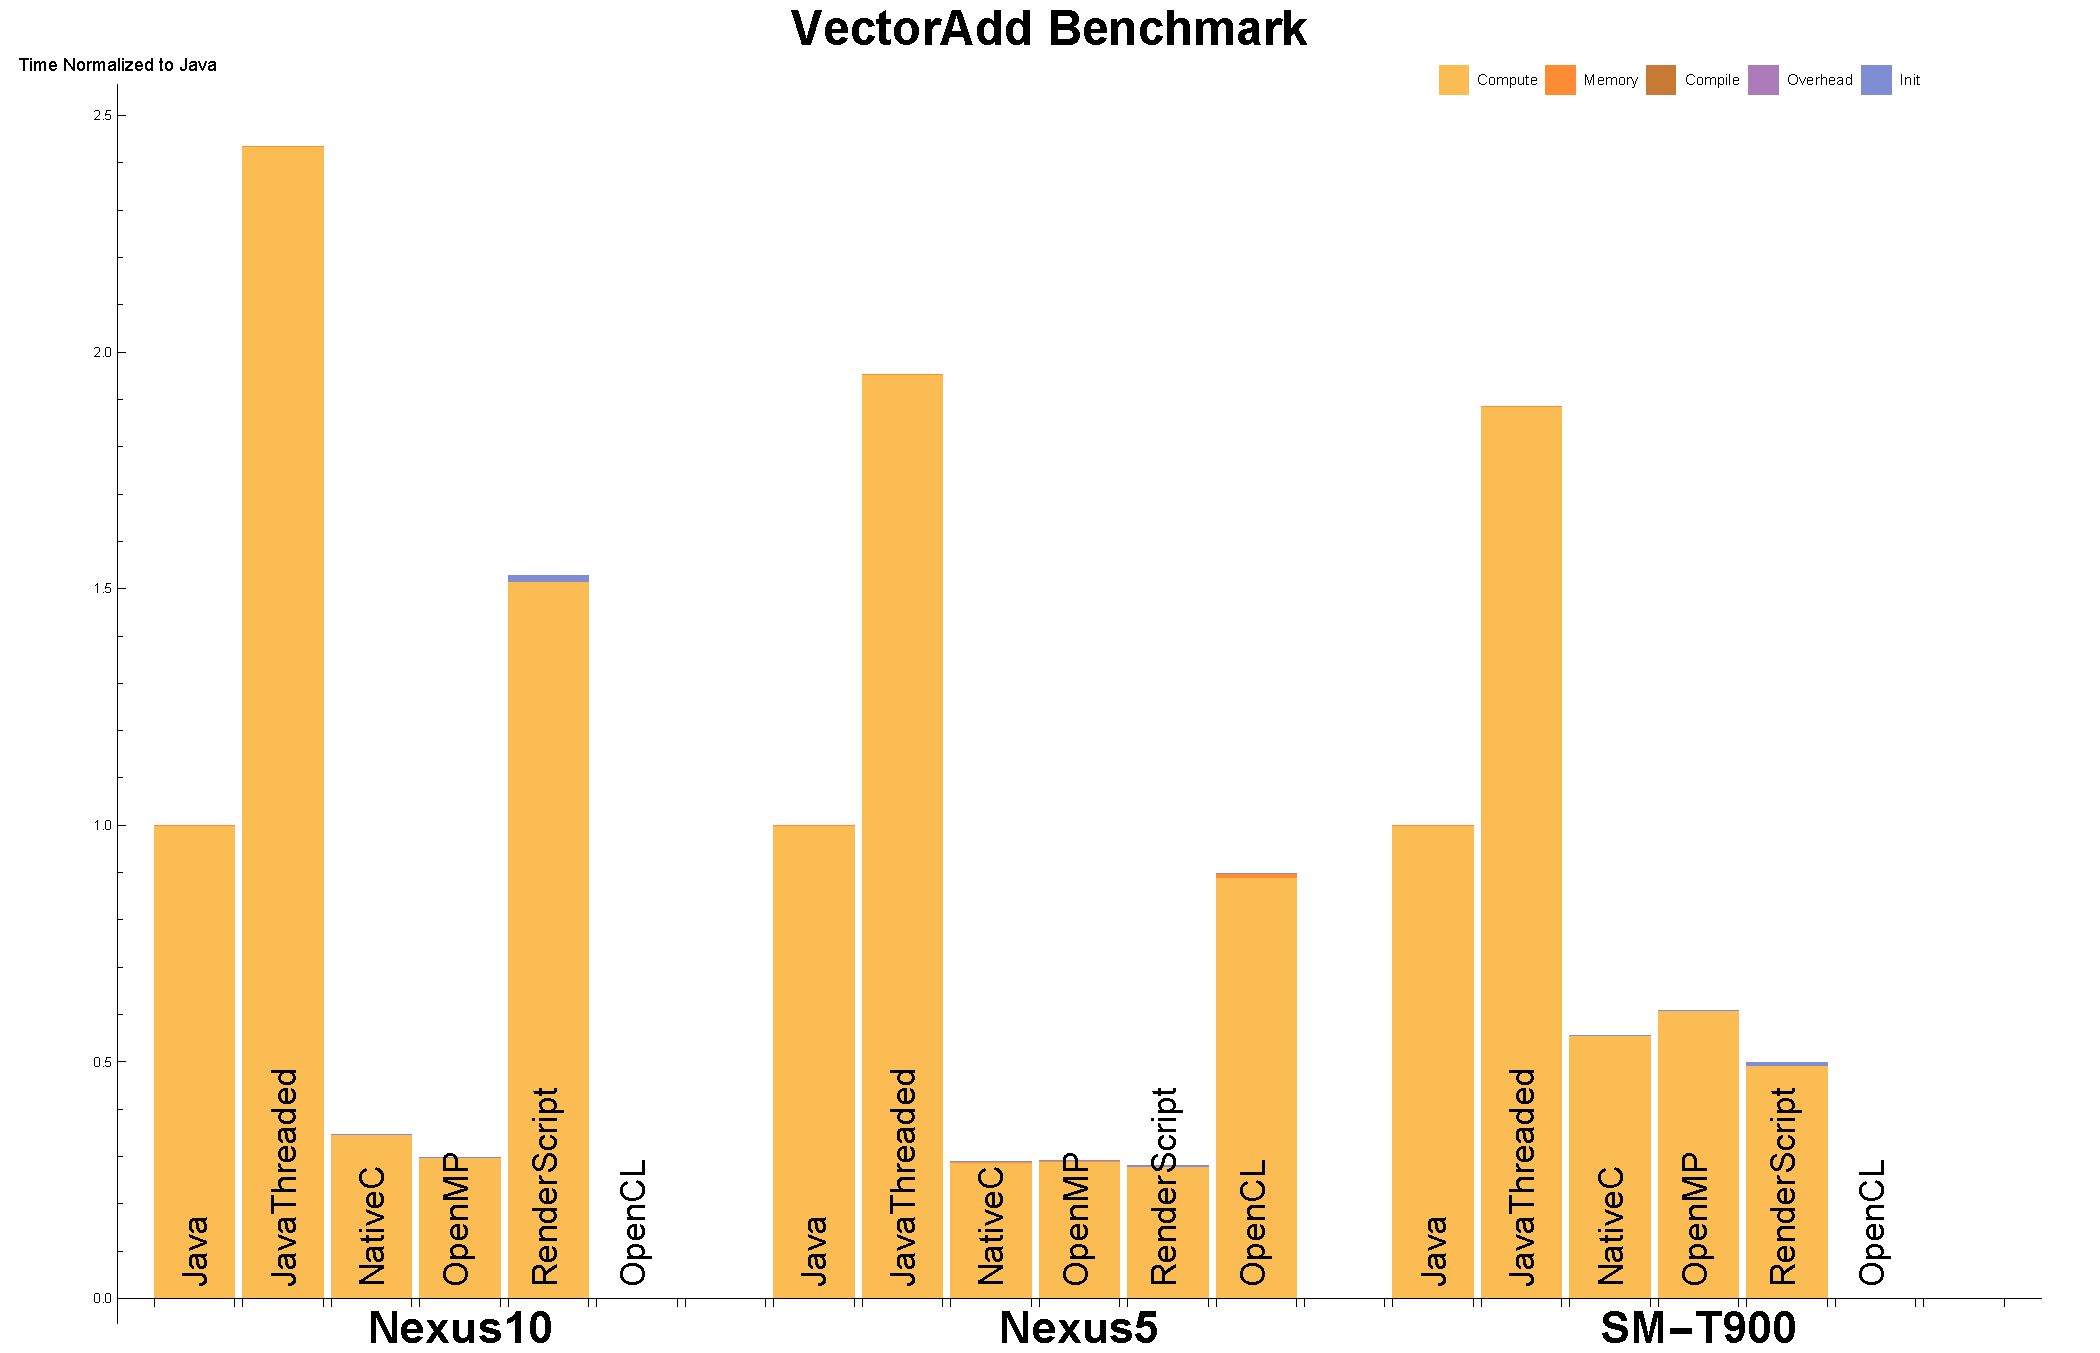
\includegraphics[width=0.9\textwidth]{data/VectorAdd_onecompute_time.pdf}
      \caption{VectorAdd}
  \end{subfigure}
  \begin{subfigure}[b]{0.33\textwidth}
      \centering
      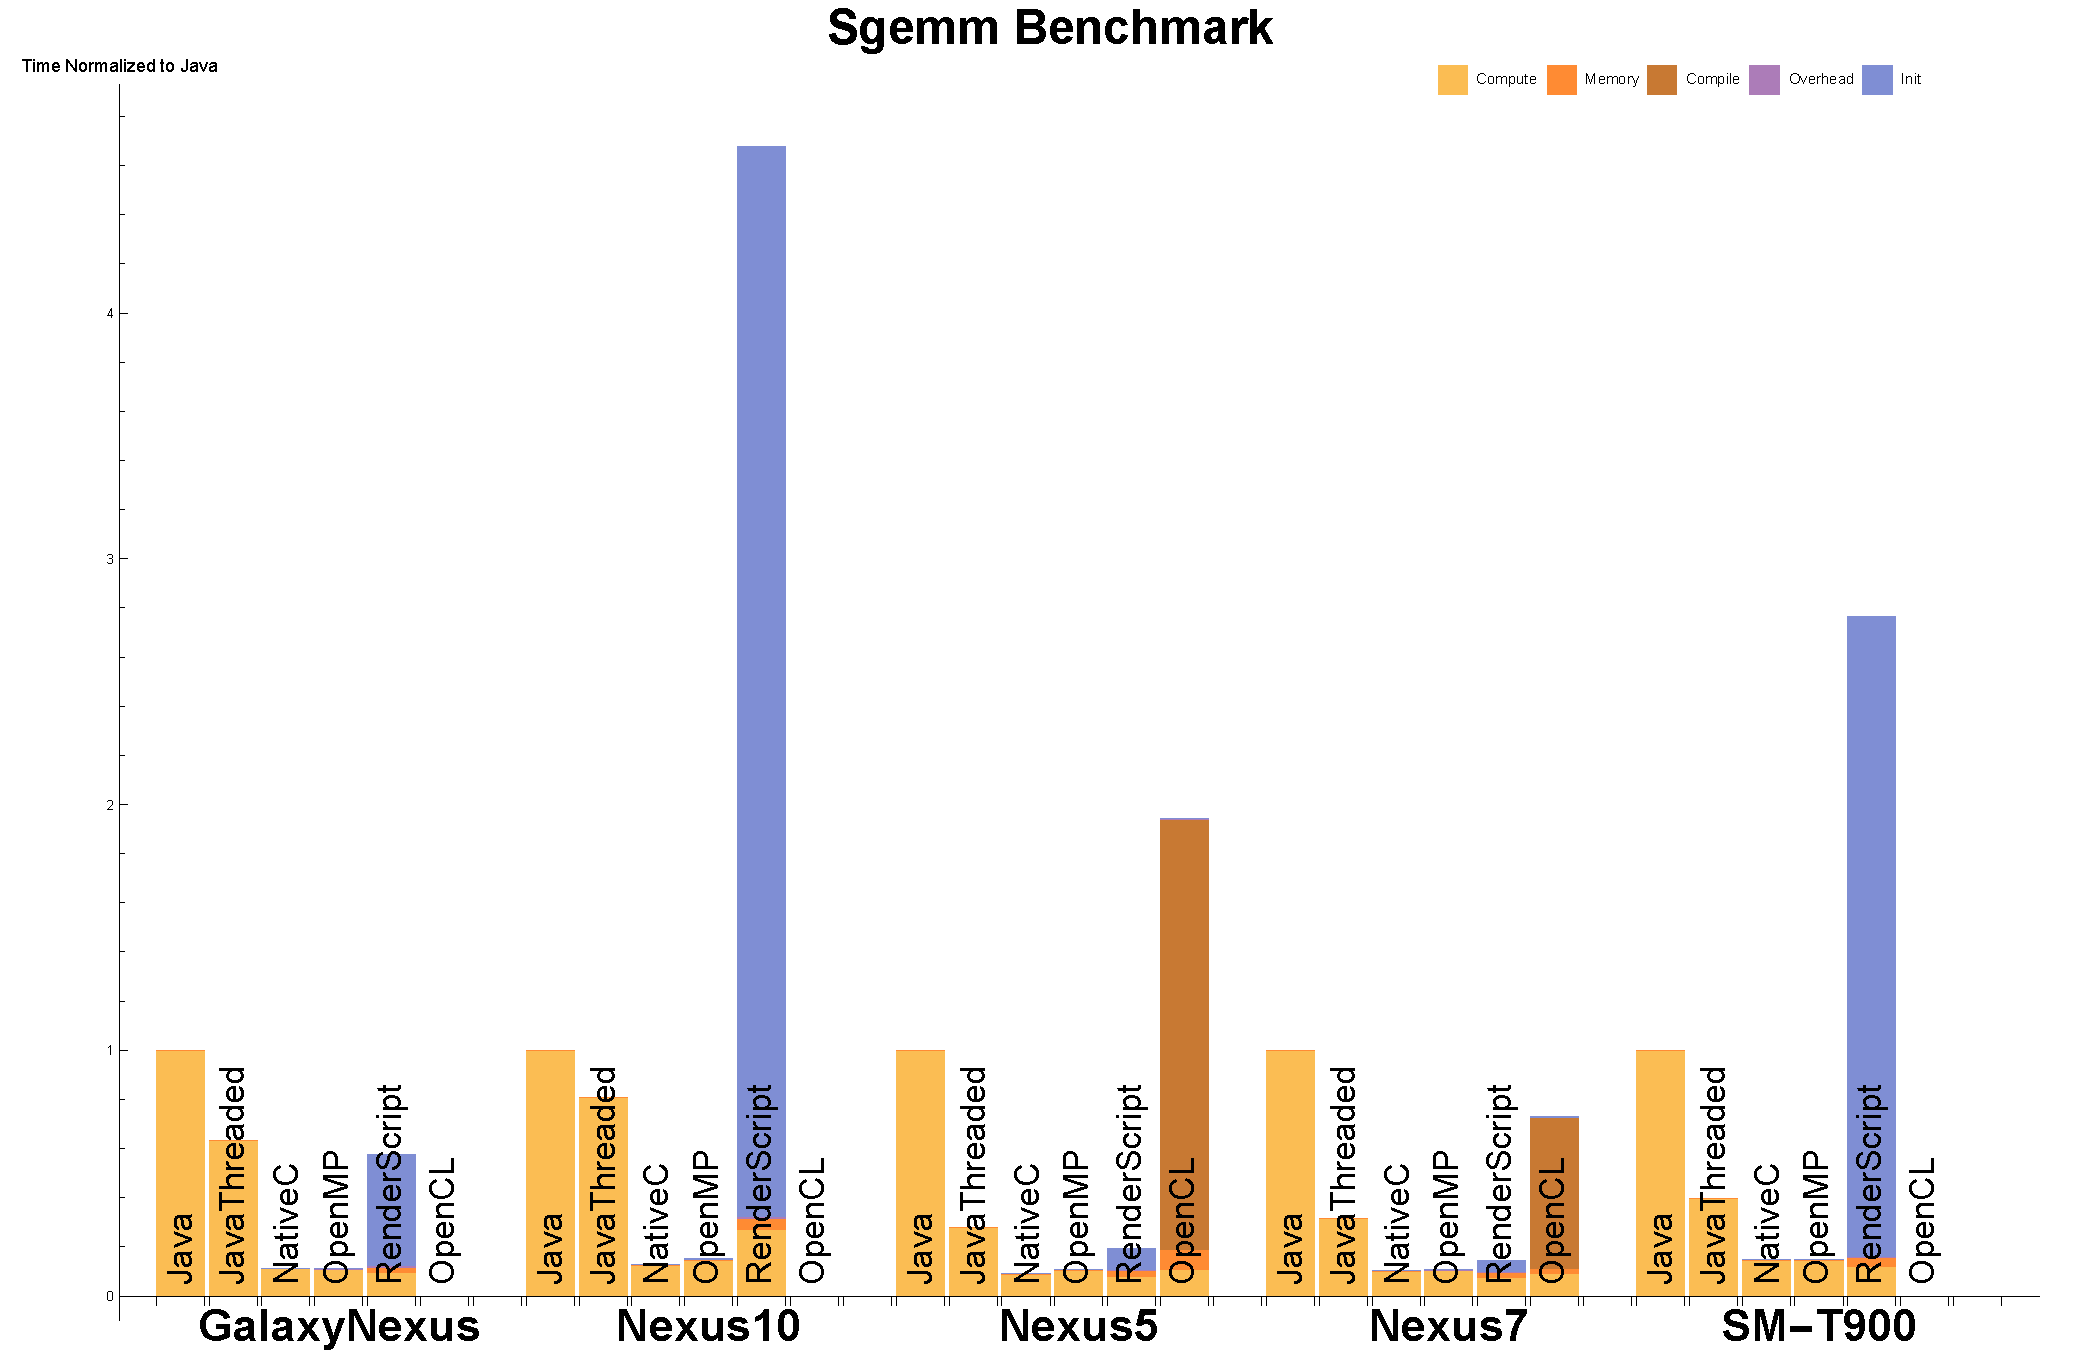
\includegraphics[width=0.9\textwidth]{data/Sgemm_onecompute_time.pdf}
      \caption{Sgemm}
  \end{subfigure}
  \begin{subfigure}[b]{0.33\textwidth}
      \centering
      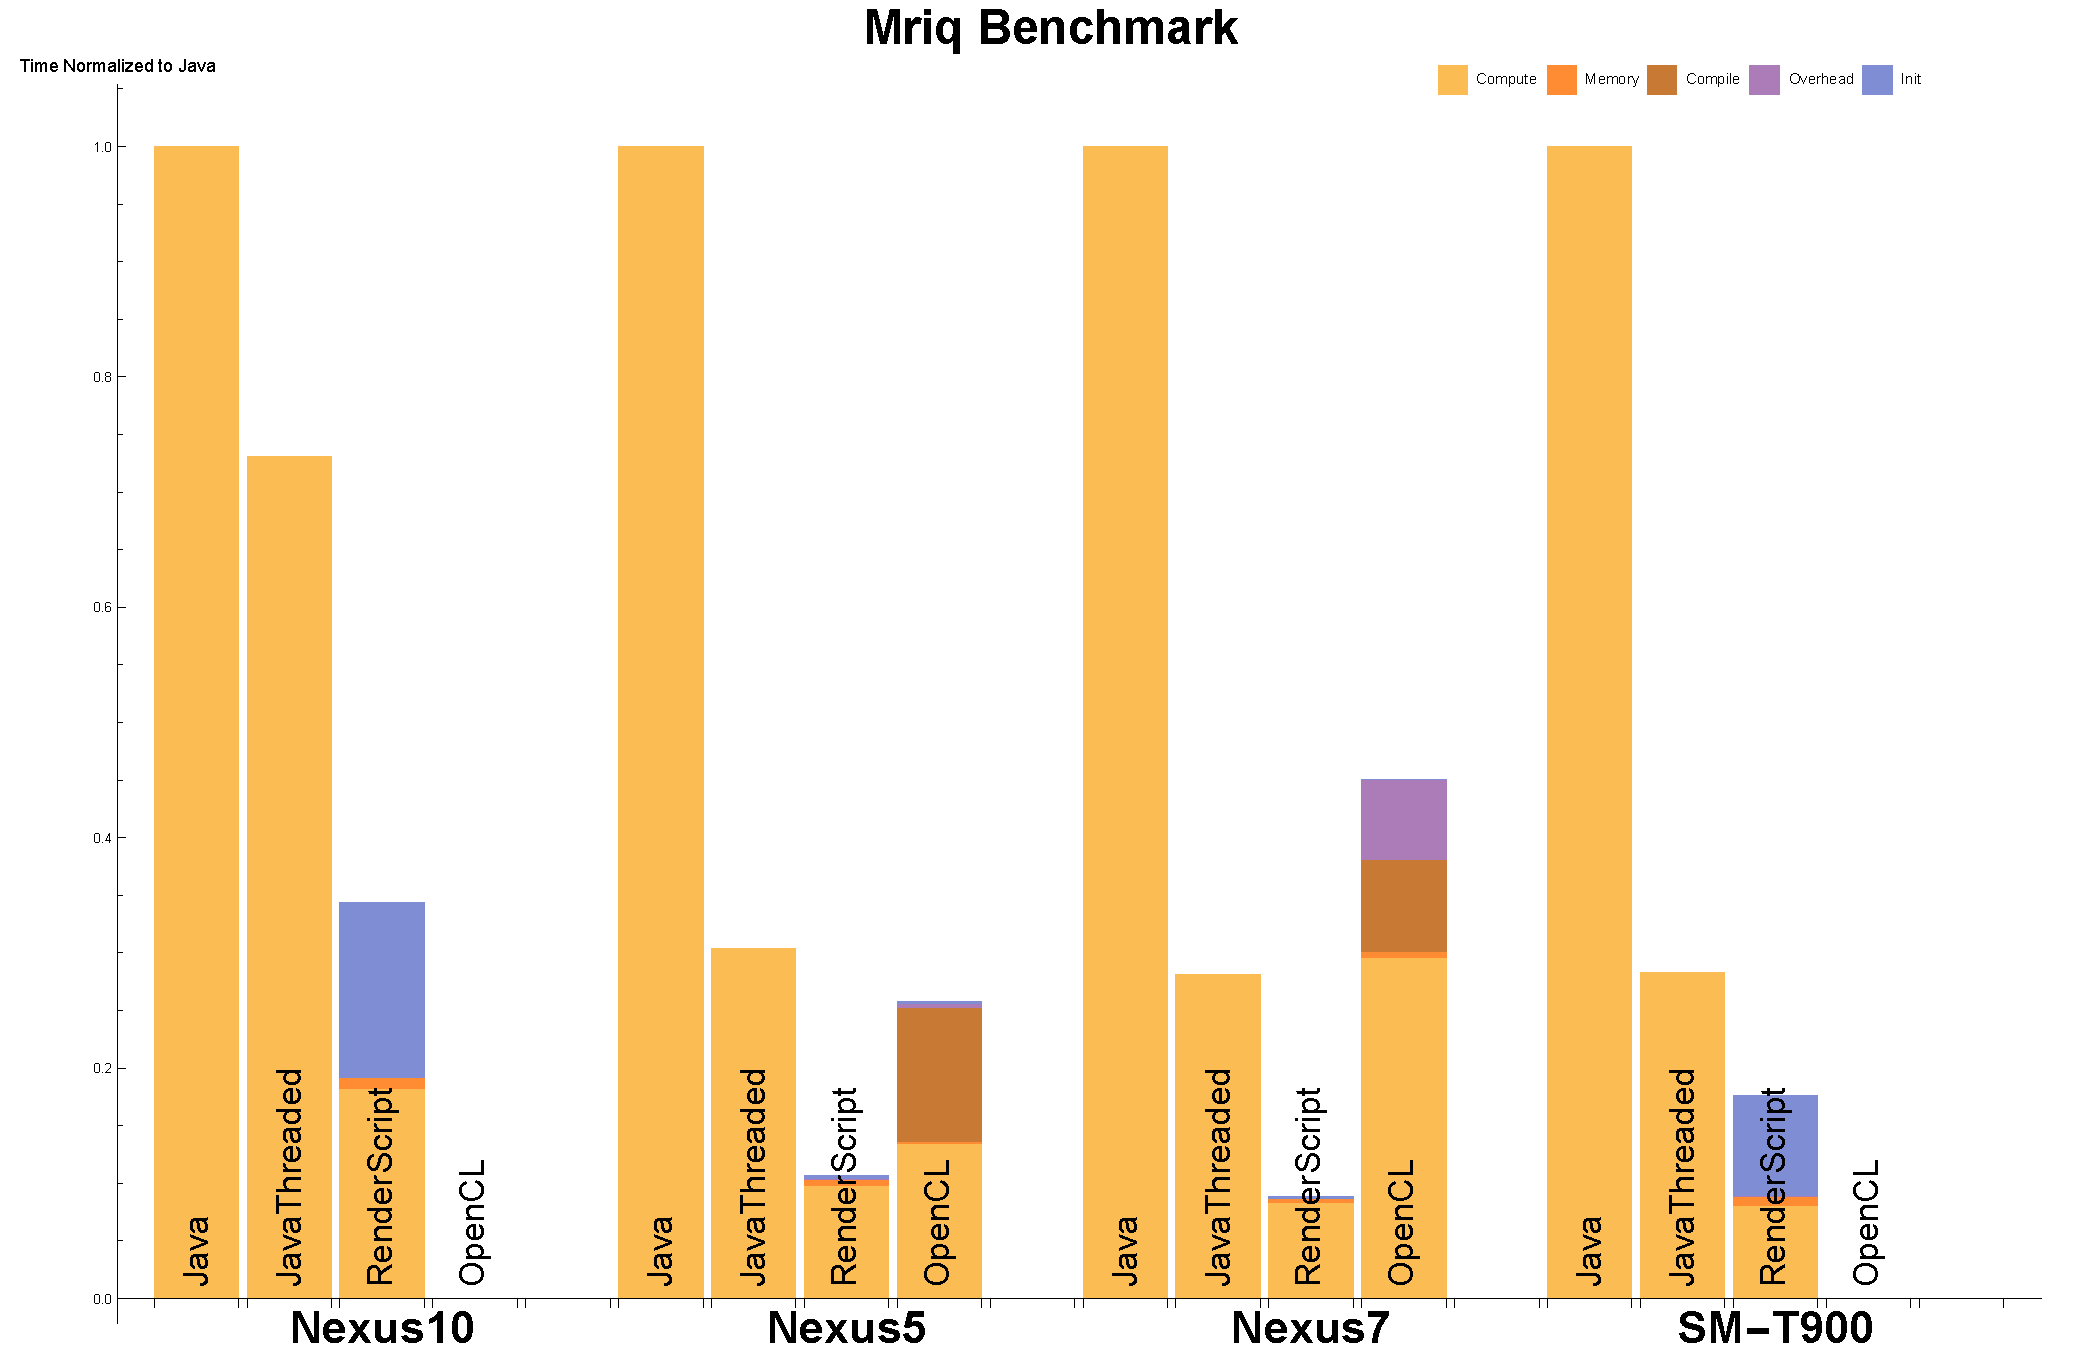
\includegraphics[width=0.9\textwidth]{data/Mriq_onecompute_time.pdf}
      \caption{MRIQ}
  \end{subfigure}

  \begin{subfigure}[b]{0.33\textwidth}
      \centering
      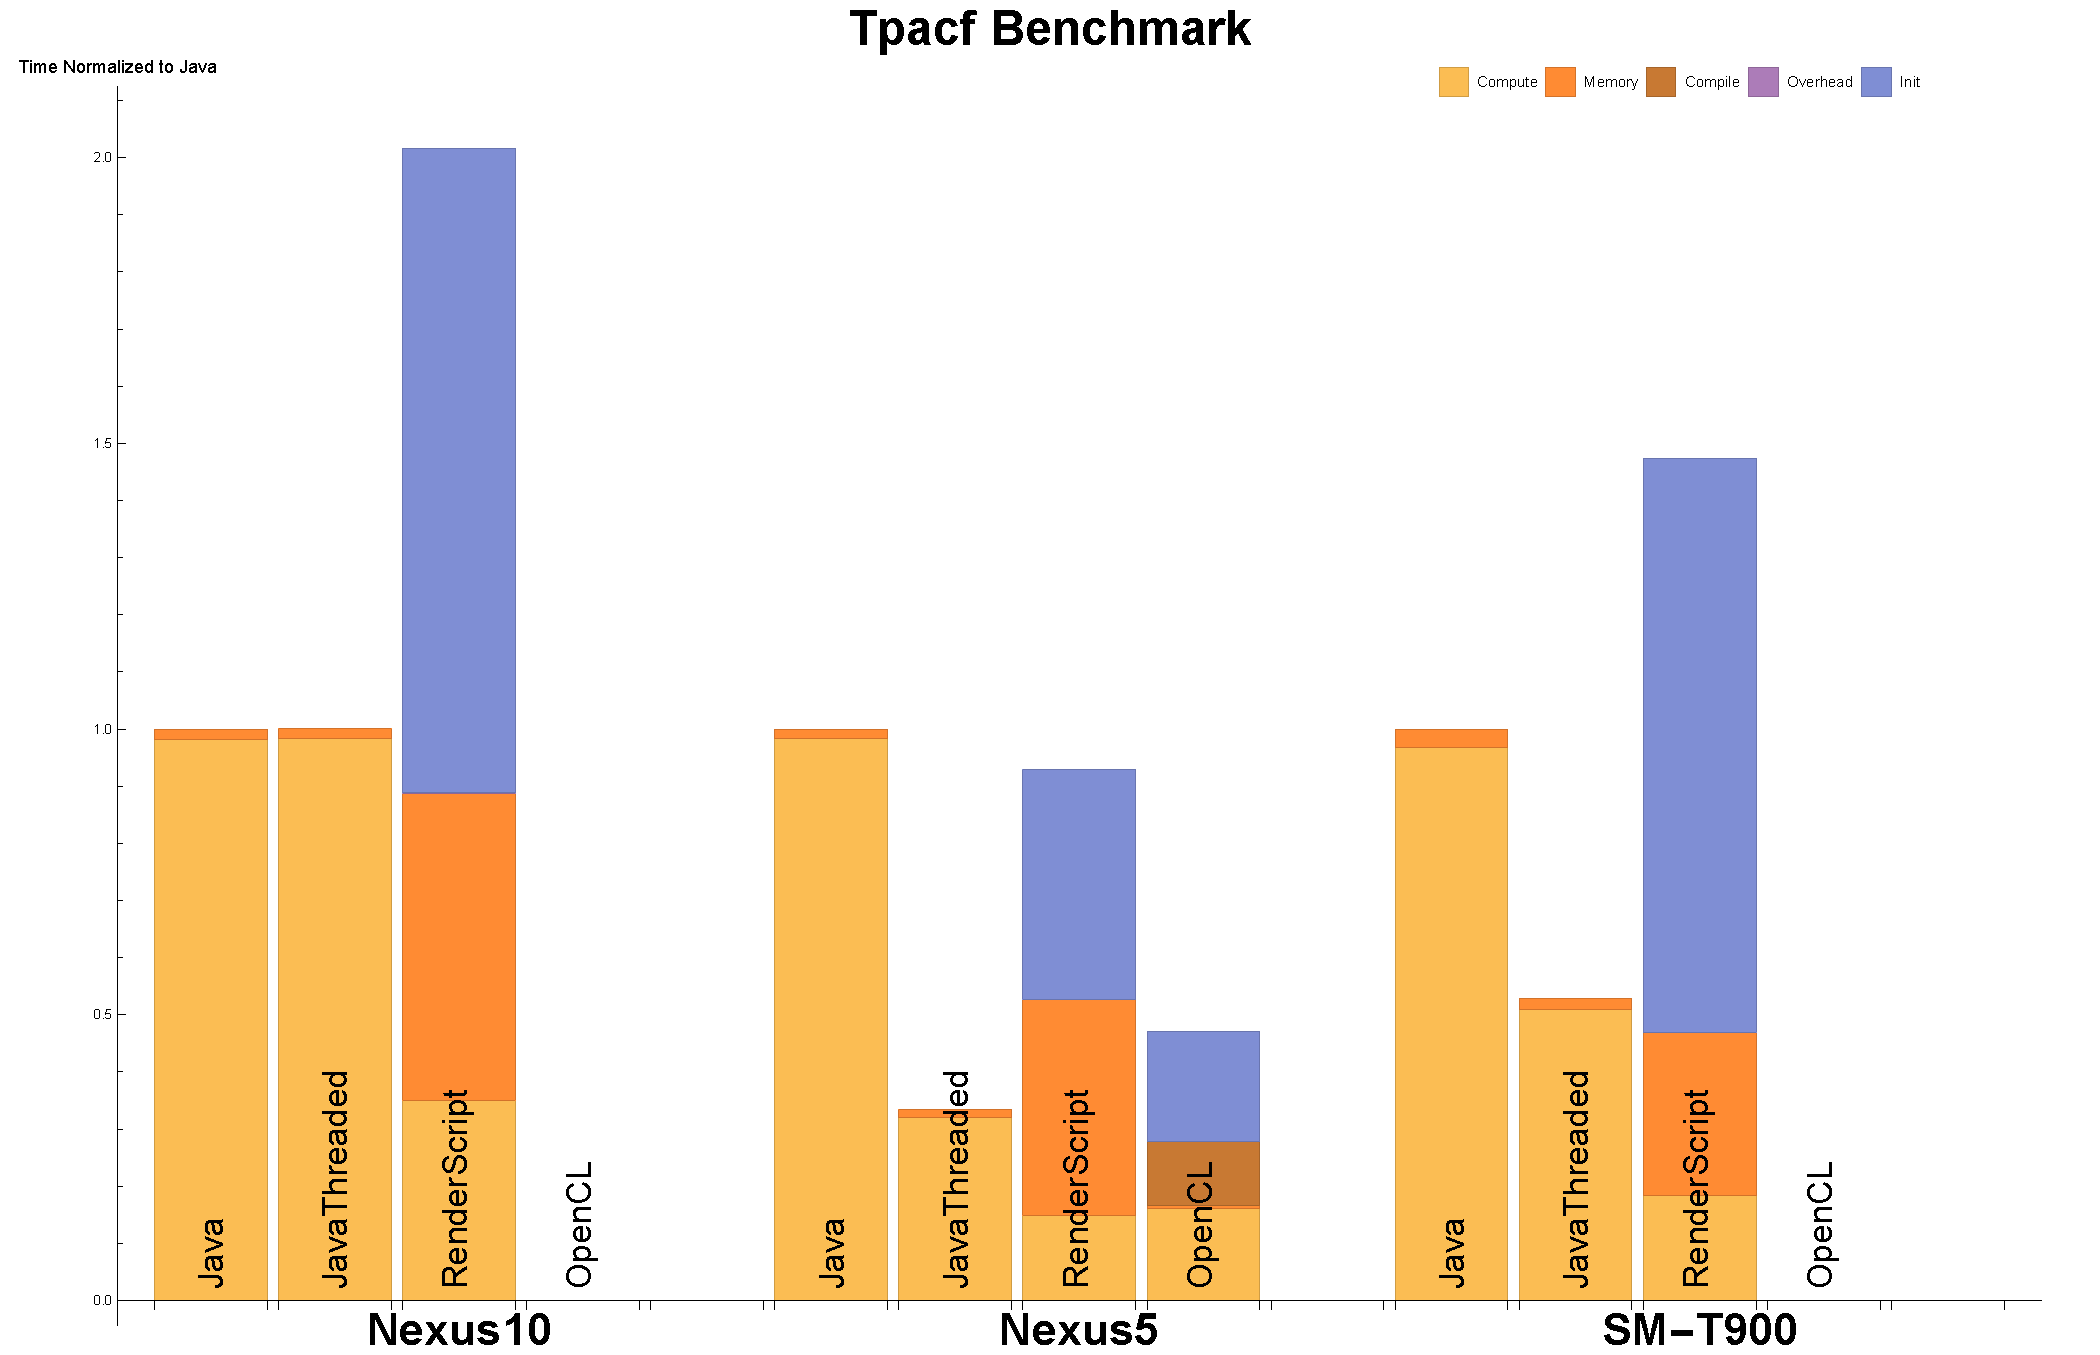
\includegraphics[width=0.9\textwidth]{data/Tpacf_onecompute_time.pdf}
      \caption{TPACF}
  \end{subfigure}
  \begin{subfigure}[b]{0.33\textwidth}
      \centering
      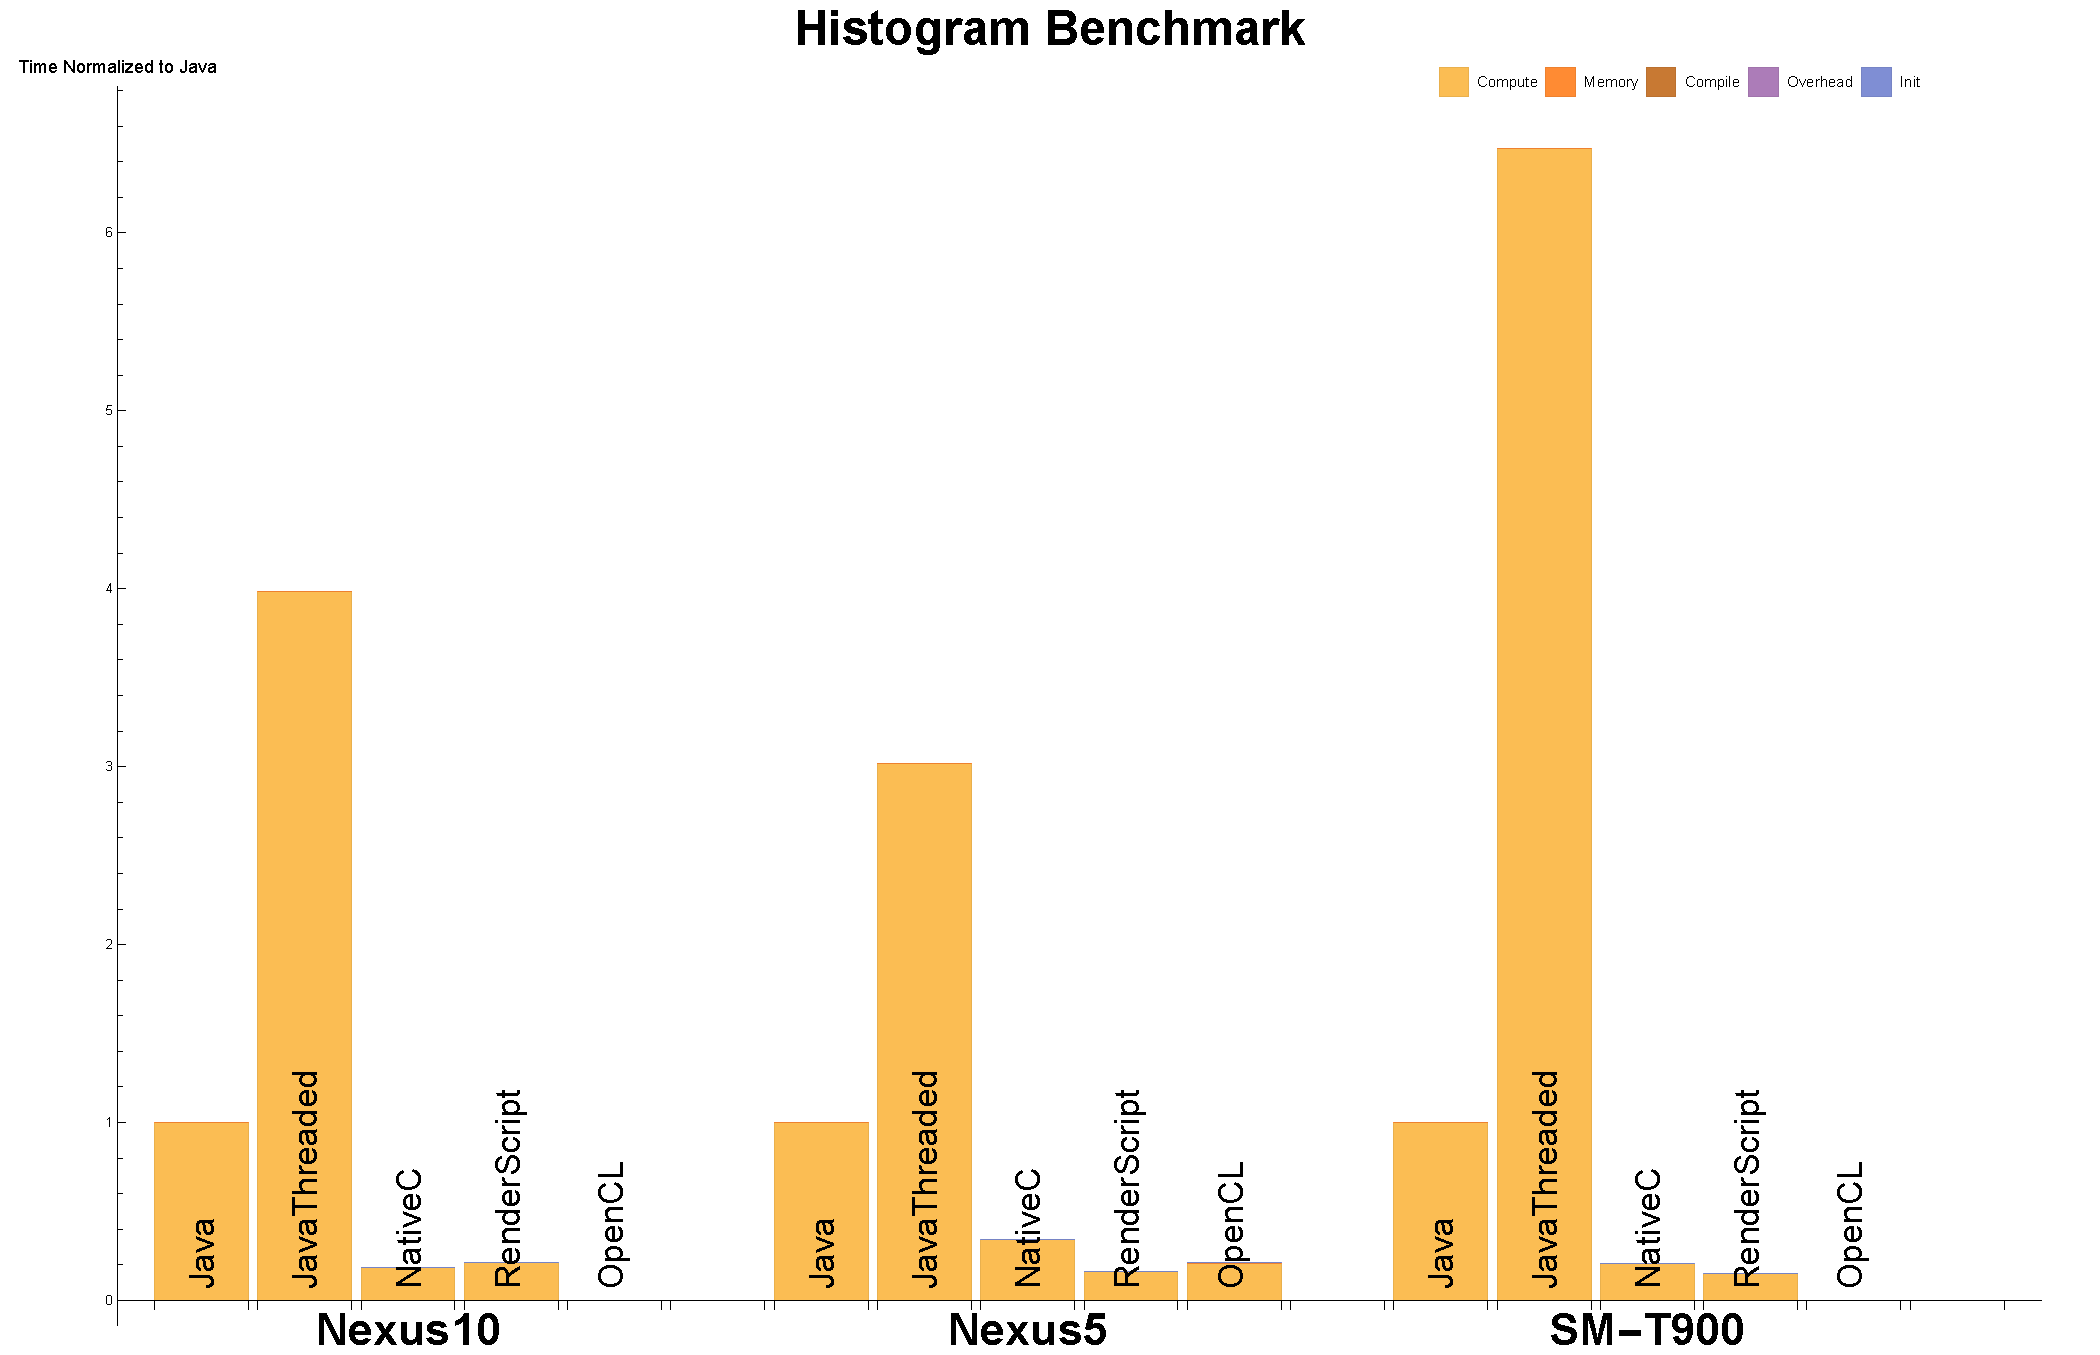
\includegraphics[width=0.9\textwidth]{data/Histogram_onecompute_time.pdf}
      \caption{Histogram}
  \end{subfigure}
  \begin{subfigure}[b]{0.33\textwidth}
      \centering
      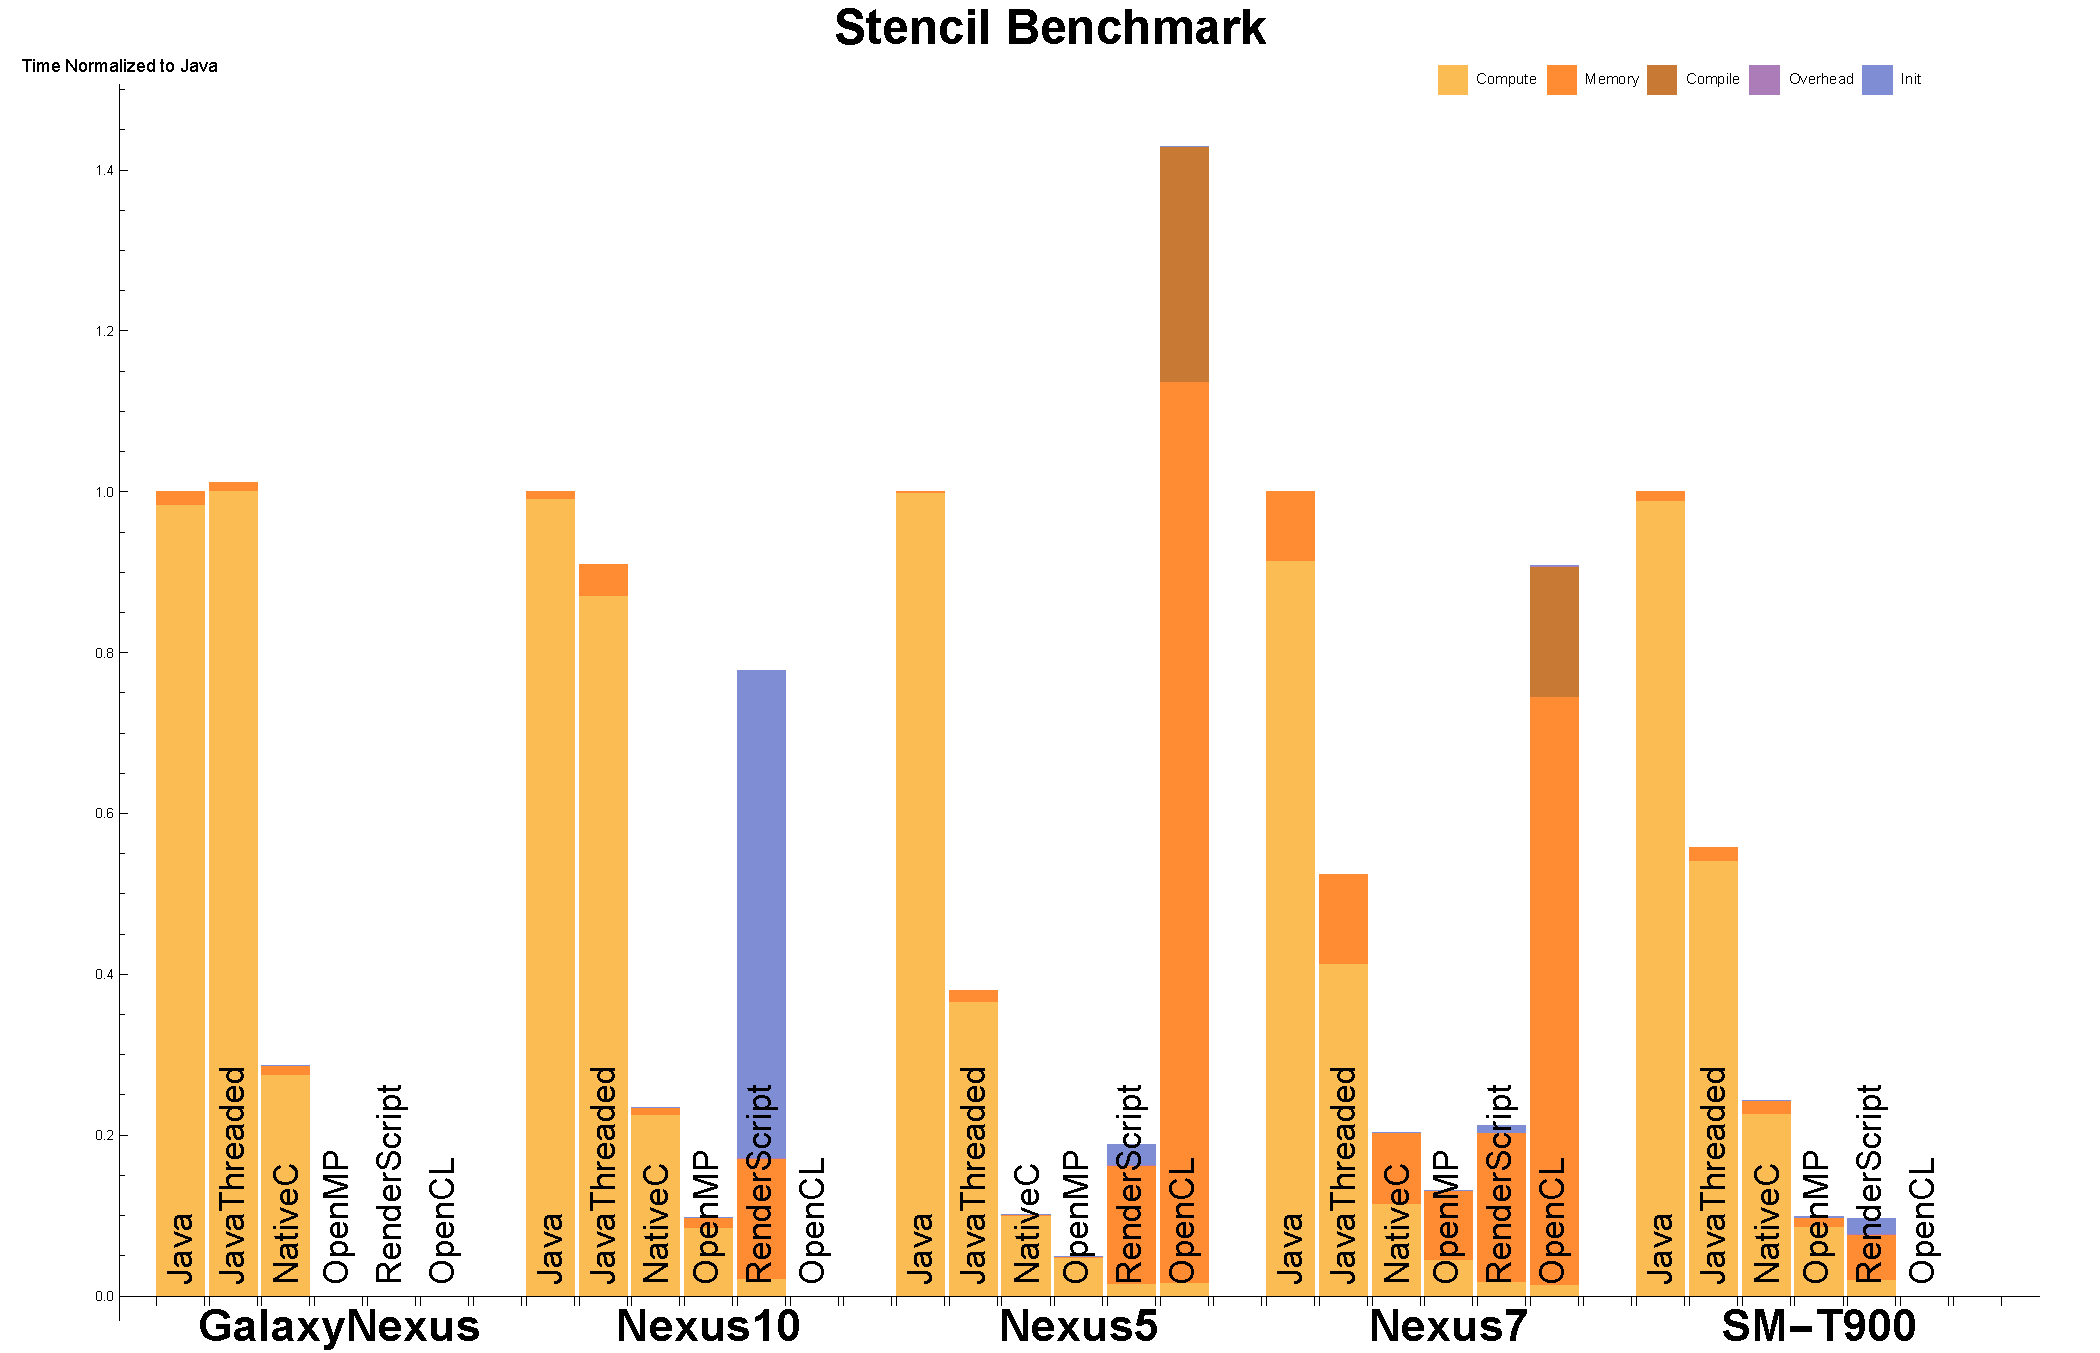
\includegraphics[width=0.9\textwidth]{data/Stencil_onecompute_time.pdf}
      \caption{Stencil}
  \end{subfigure}
  \caption{Runtime across devices where kernel is executed once. The runtime is normalized to the Java execution time (lower is better). J : Java, JT : JavaThreaded, C : Native C, OMP: OpenMP, OCL : OpenCL, and RS : RenderScript.}
  \label{fig:perfOne}
\end{figure*}

\begin{figure*}

  \centering
  \begin{subfigure}[b]{\textwidth}
          \centering
          
\includegraphics[width=0.4\textwidth]{data/legend.pdf}
  \end{subfigure}

  \begin{subfigure}[b]{0.33\textwidth}
      \centering
      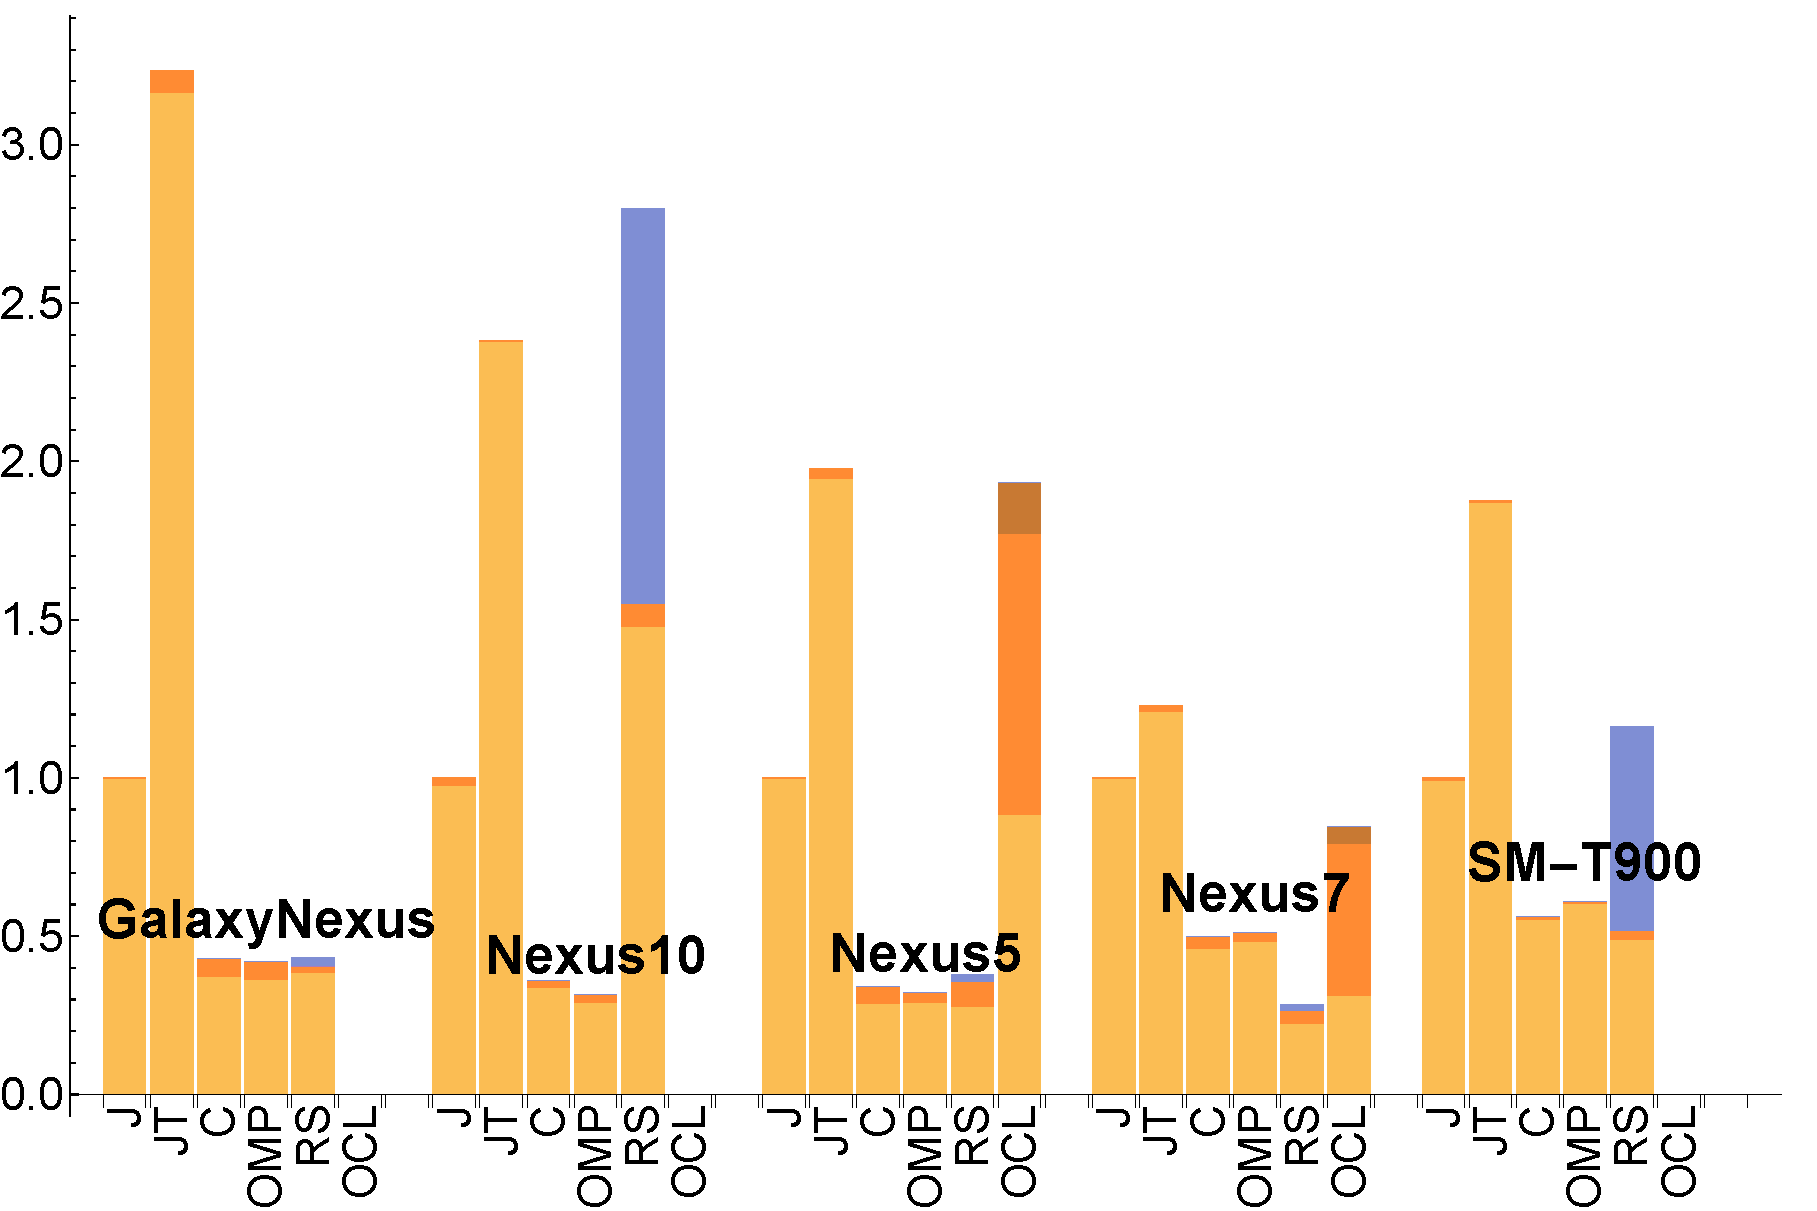
\includegraphics[width=0.9\textwidth]{data/VectorAdd_time.pdf}
      \caption{VectorAdd}
  \end{subfigure}
  \begin{subfigure}[b]{0.33\textwidth}
      \centering
      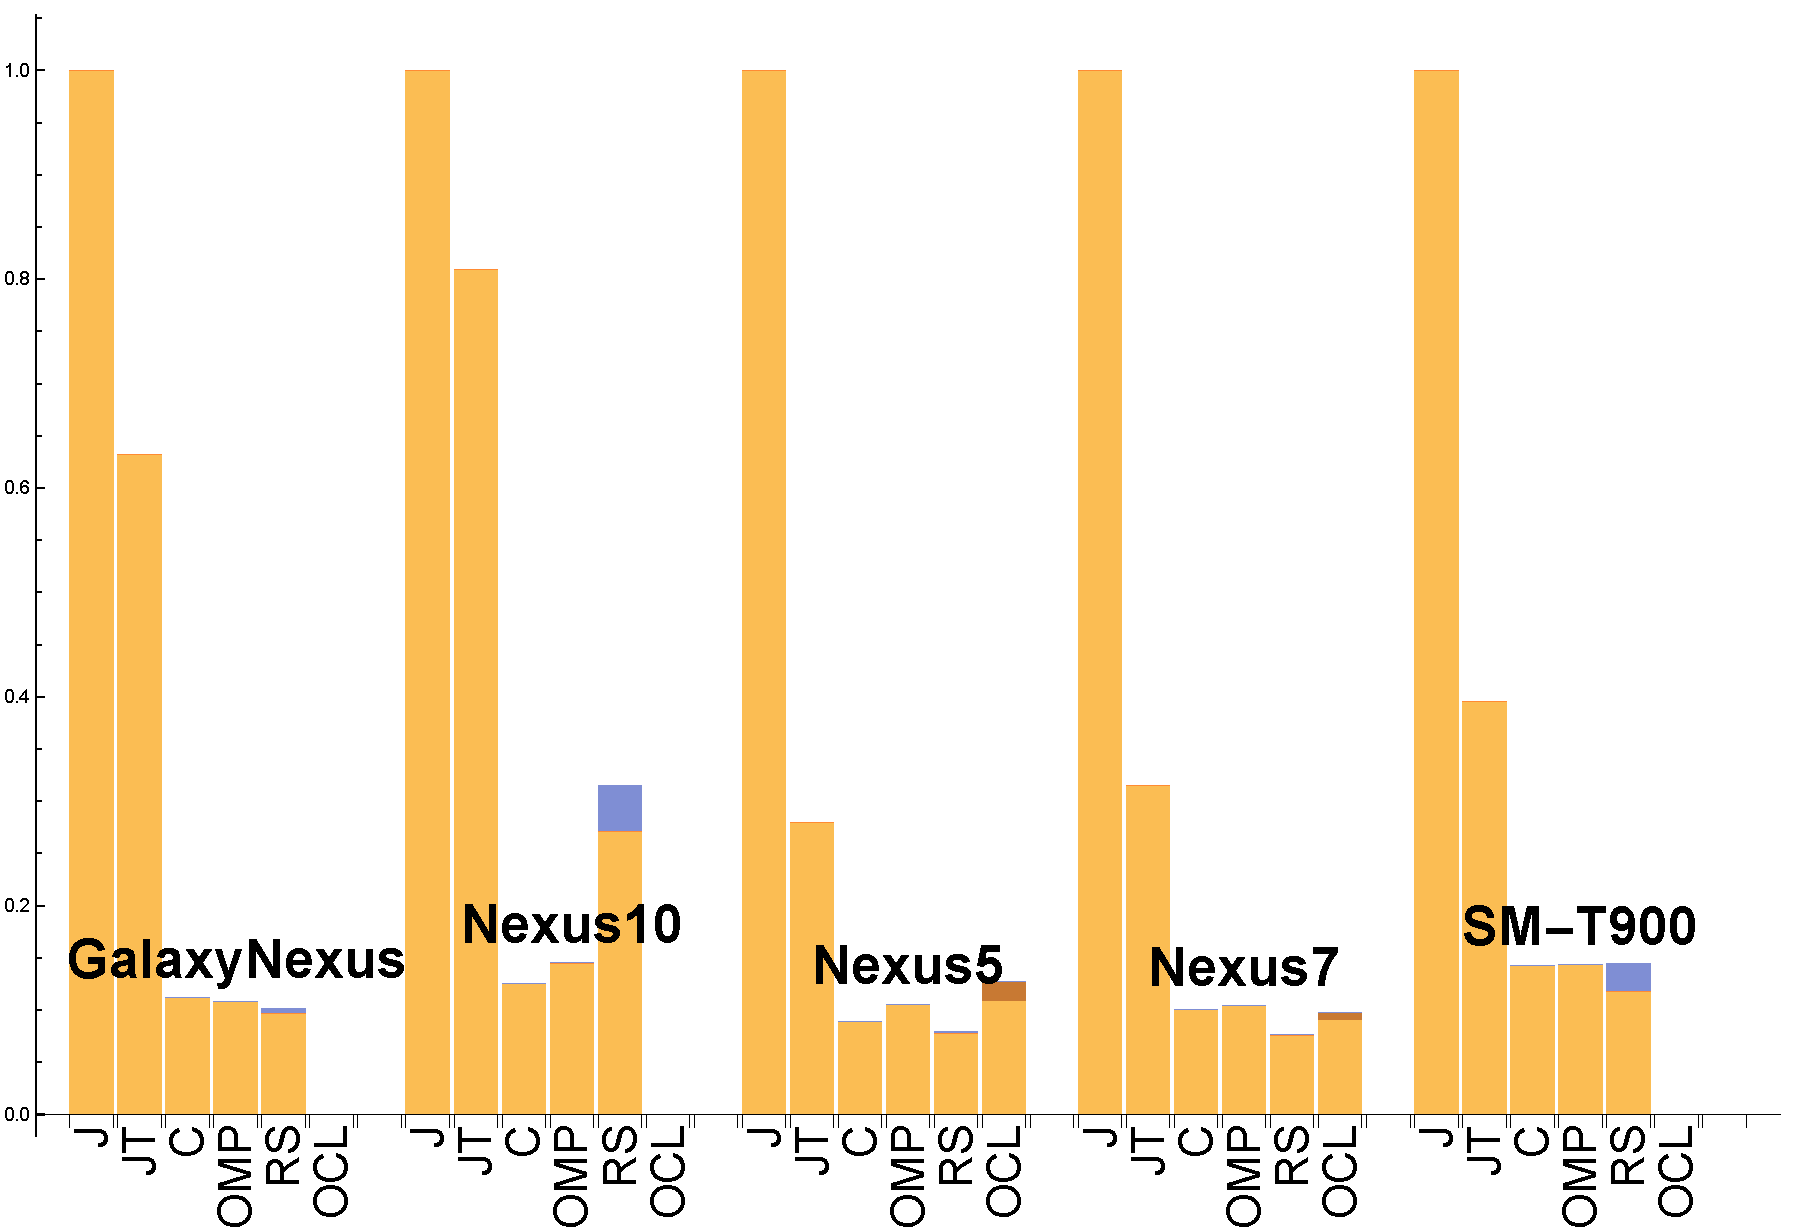
\includegraphics[width=0.9\textwidth]{data/Sgemm_time.pdf}
      \caption{Sgemm}
  \end{subfigure}
  \begin{subfigure}[b]{0.33\textwidth}
      \centering
      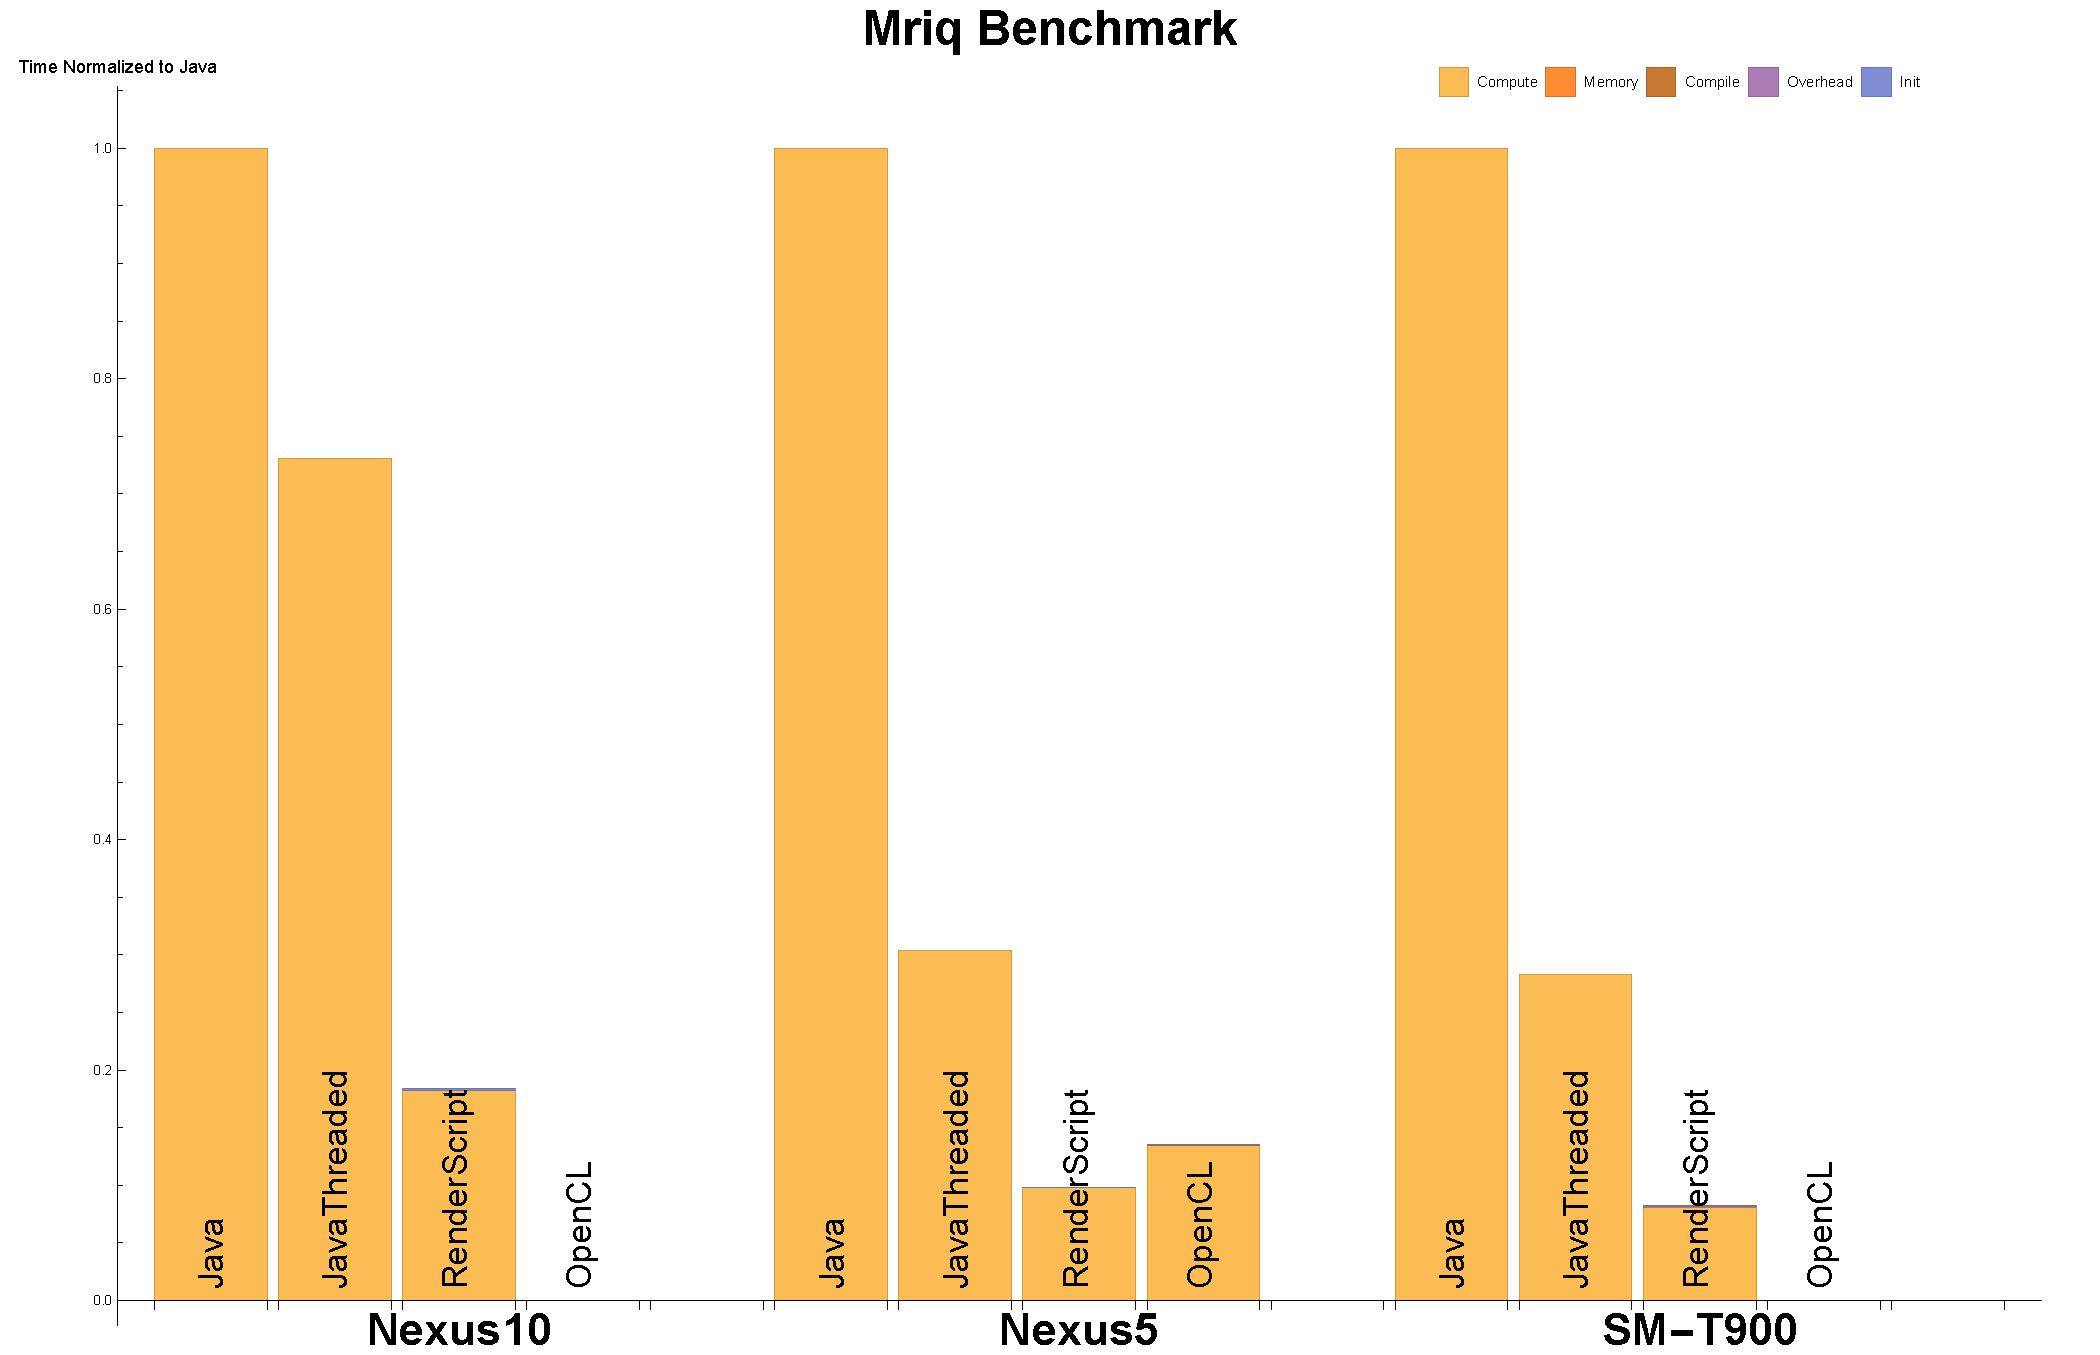
\includegraphics[width=0.9\textwidth]{data/Mriq_time.pdf}
      \caption{MRIQ}
  \end{subfigure}

  \begin{subfigure}[b]{0.33\textwidth}
      \centering
      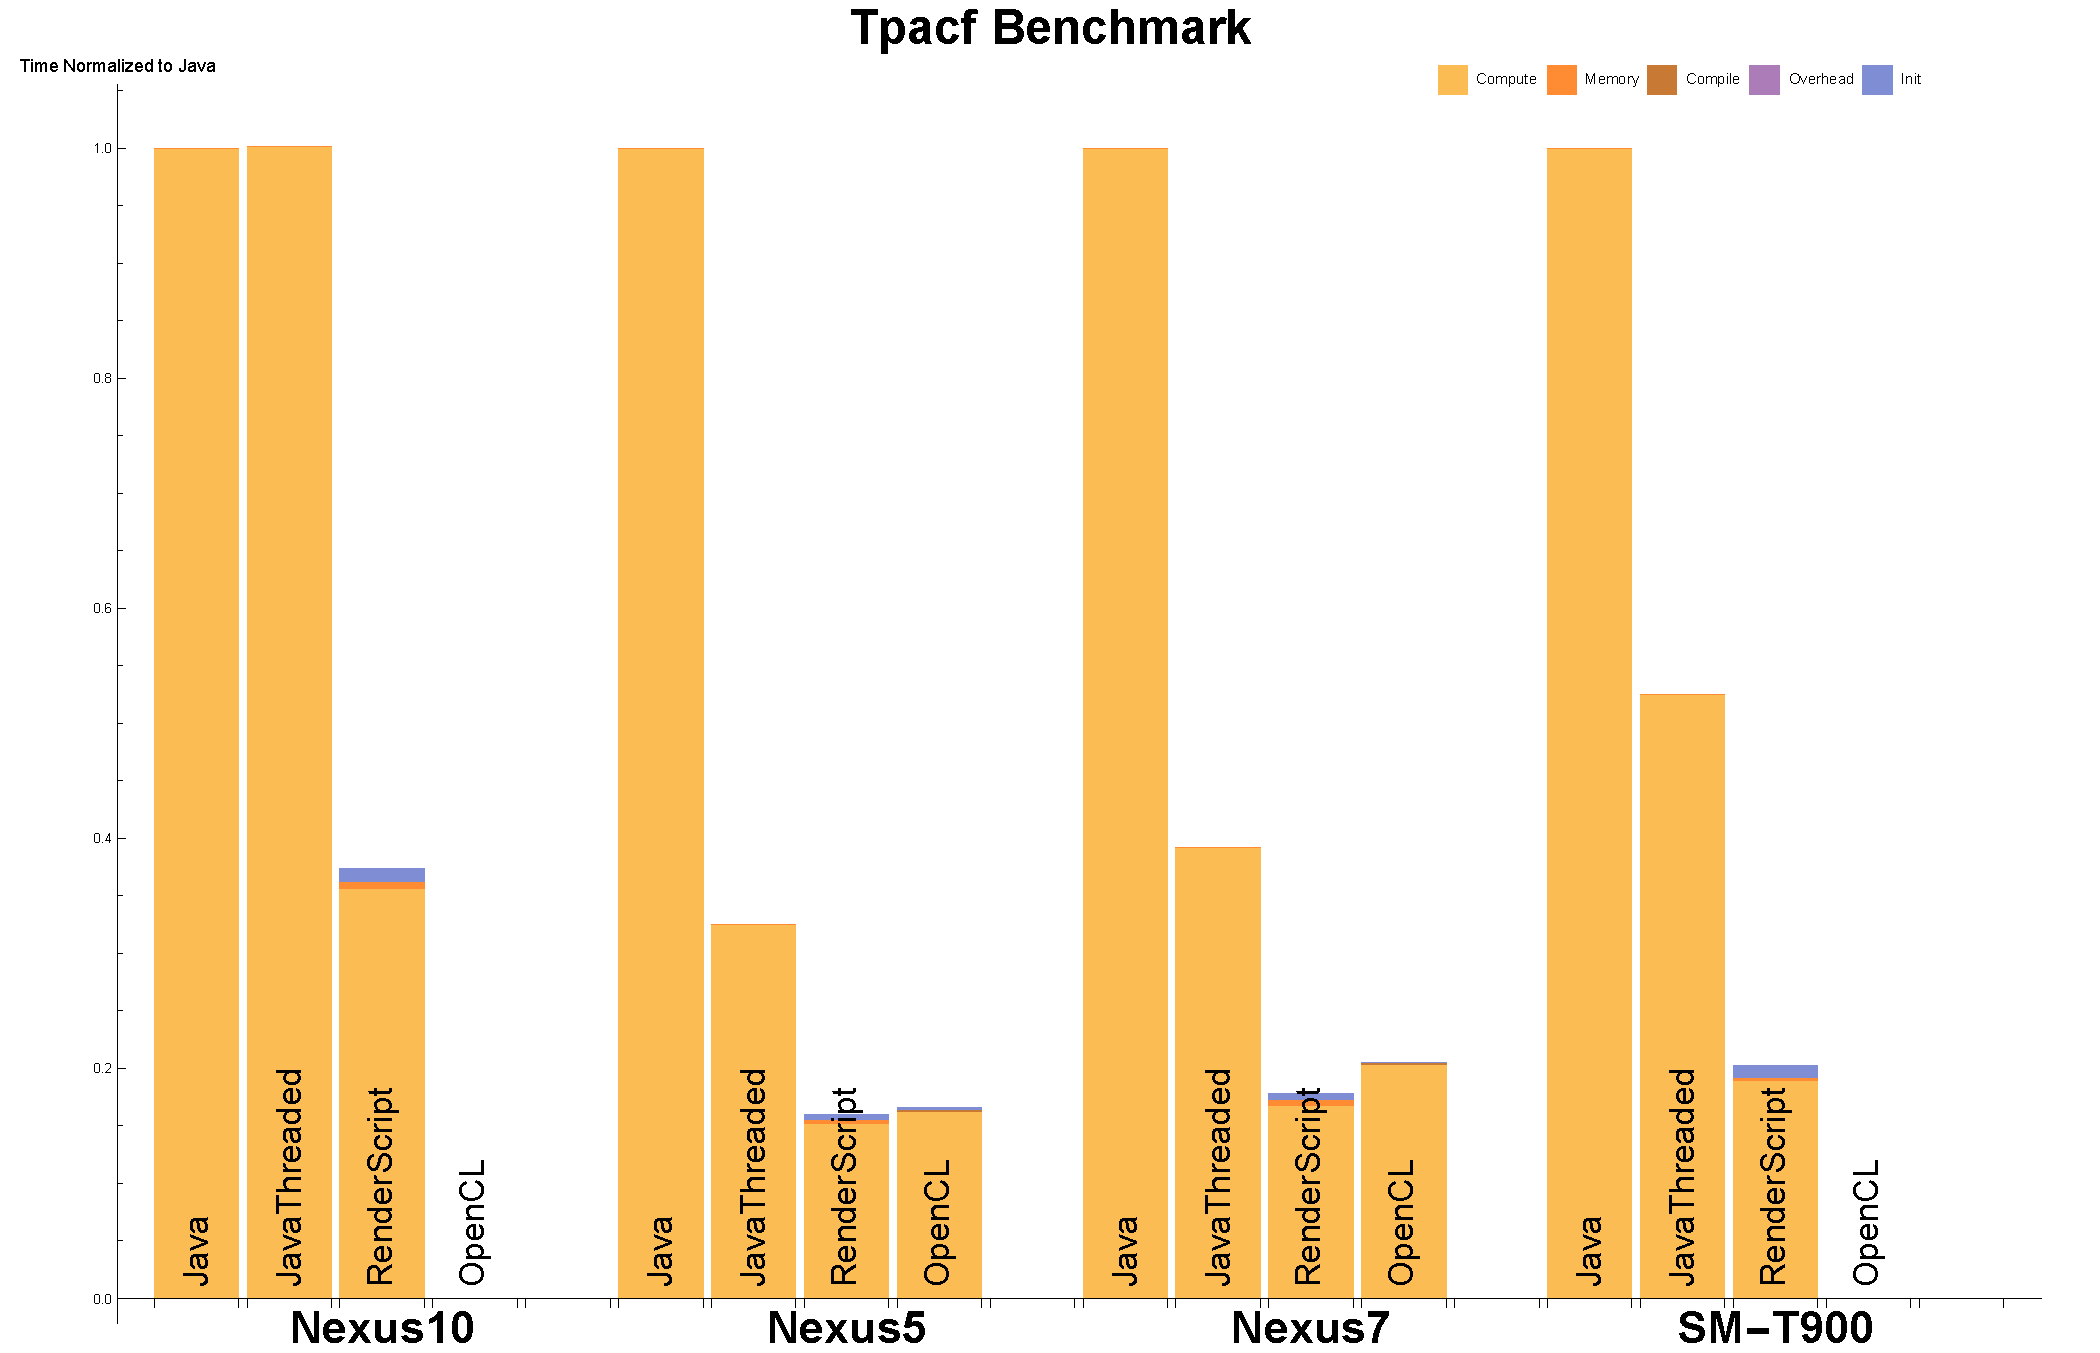
\includegraphics[width=0.9\textwidth]{data/Tpacf_time.pdf}
      \caption{TPACF}
  \end{subfigure}
  \begin{subfigure}[b]{0.33\textwidth}
      \centering
      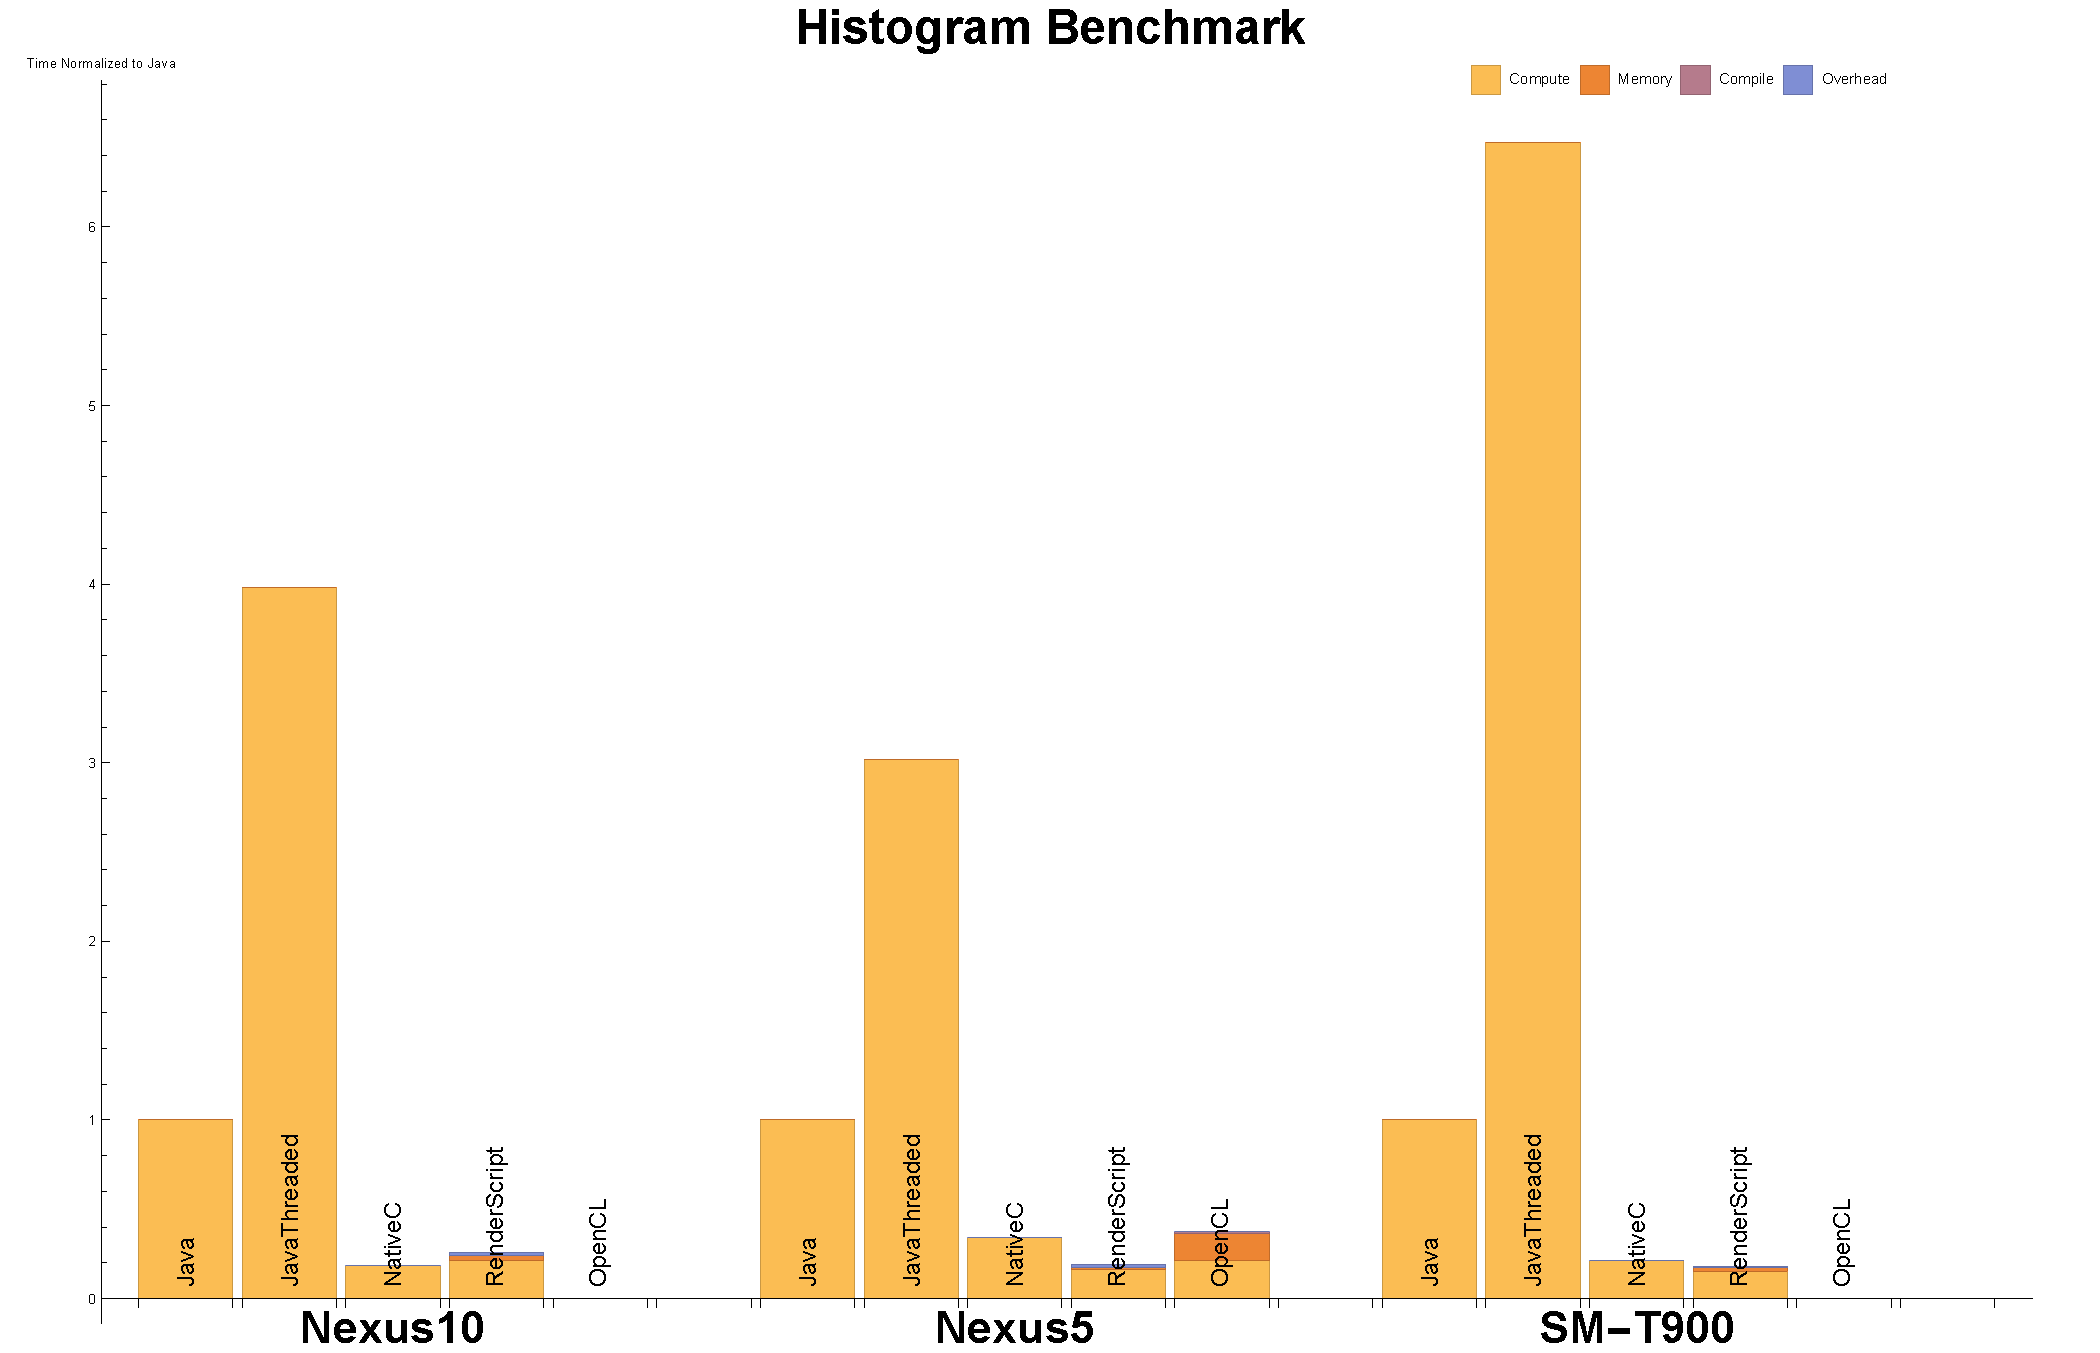
\includegraphics[width=0.9\textwidth]{data/Histogram_time.pdf}
      \caption{Histogram}
  \end{subfigure}
  \begin{subfigure}[b]{0.33\textwidth}
      \centering
      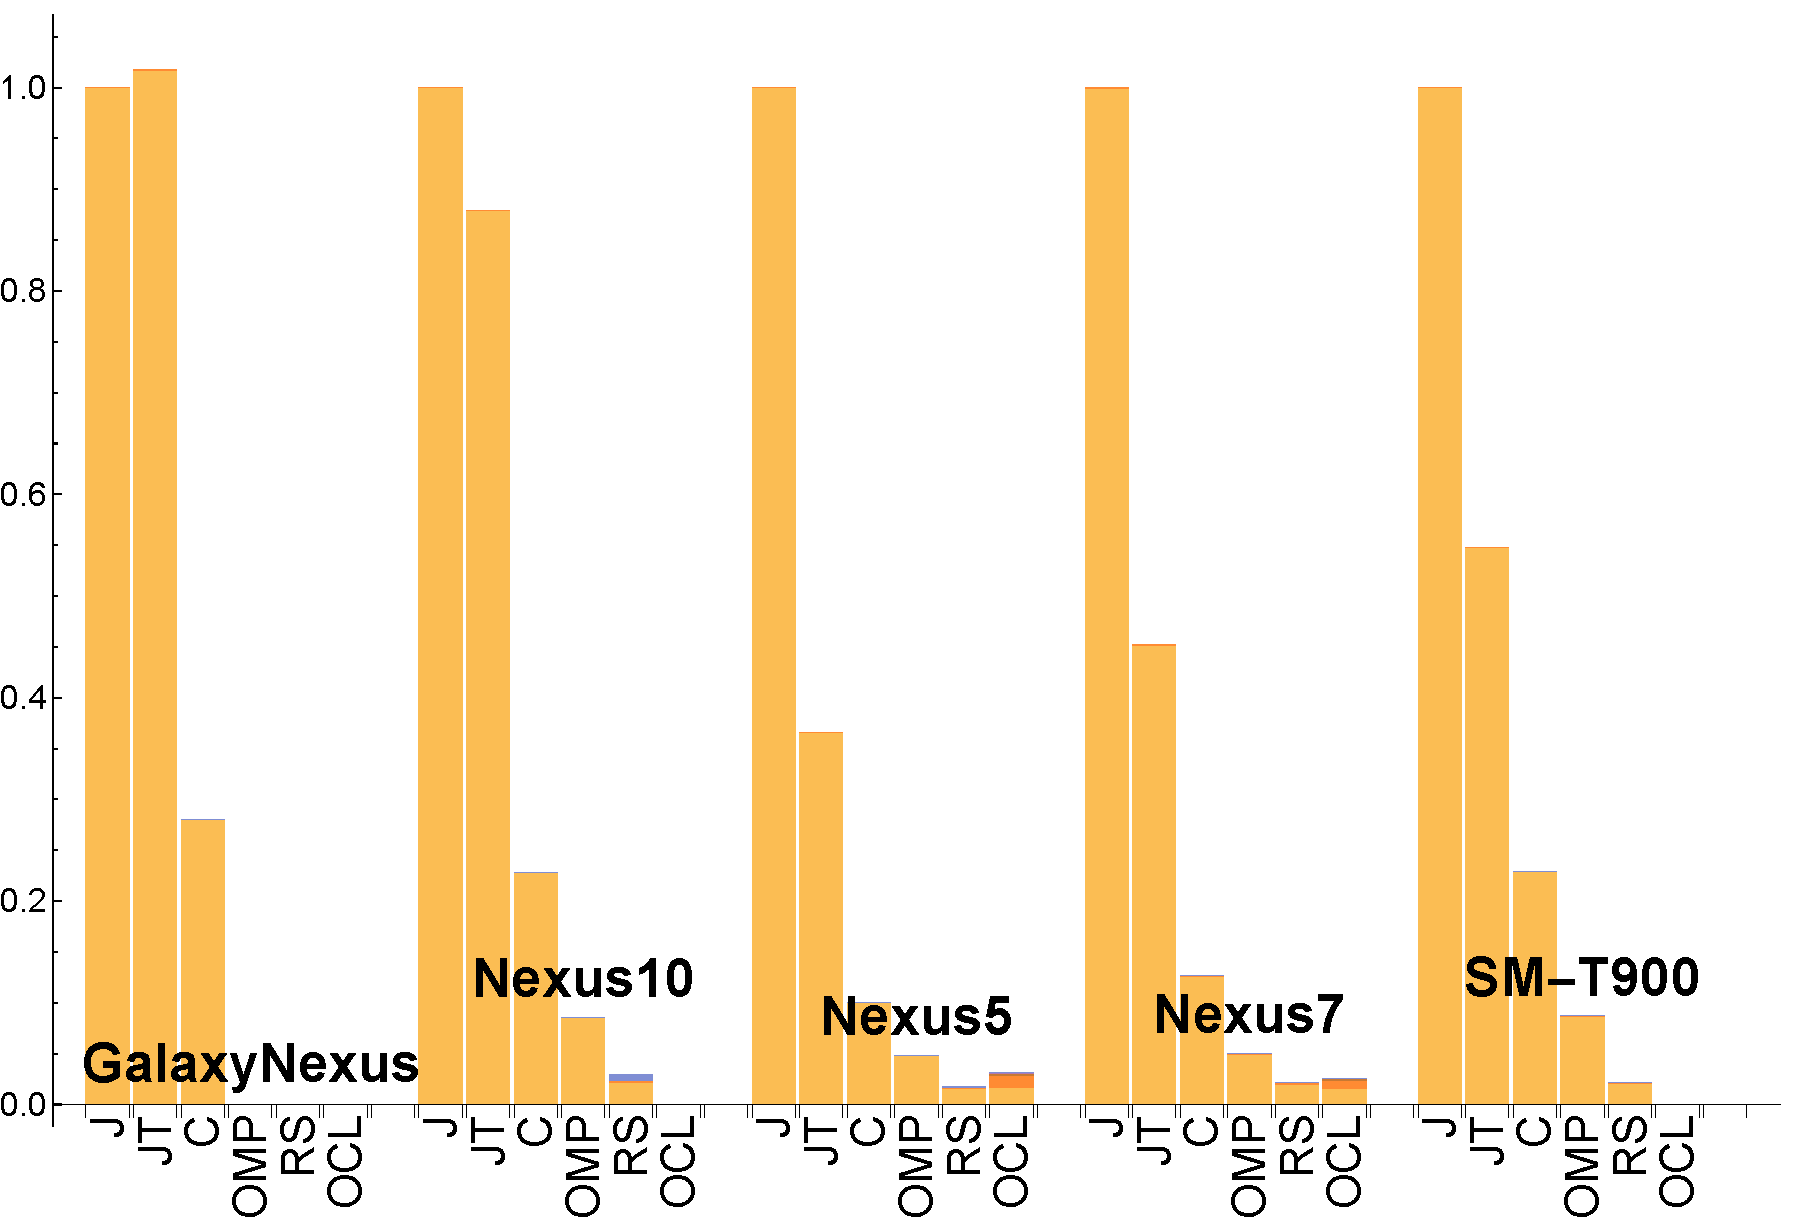
\includegraphics[width=0.9\textwidth]{data/Stencil_time.pdf}
      \caption{Stencil}
  \end{subfigure}

  \caption{Runtime across devices where kernel is executed multiple times. The runtime is normalized to the Java execution time (lower is better). J : Java, JT : JavaThreaded, C : Native C, OMP: OpenMP, OCL : OpenCL, and RS : RenderScript.}
  \label{fig:perfMany}
\end{figure*}


The performance measurements are collected by measuring the time
  spent within each section of the code while the device is plugged
  into the development machine.
Each compute part of an implementation is run $5$ times with the minimum
  presented.
We consider two cases --- one where the kernel code is run once (figure~\ref{fig:perfOne}) and therefore
  the overhead (memory, compilation, and initialization) have an impact,
  and one where the kernel is run $100$ times (figure~\ref{fig:perfMany}) (or $5$ for both TPACF and MRIQ)
  and the overhead has little impact.

For each device, the plot show the time to execute sections of the code normalized
  to the Java execution time.
These times correspond to the $x$-axis of the processor utilization times discussed
  in the previous section (e.g. figure~\ref{fig:loadVecAddSgemm}) --- Trepn is not
  running while collecting these timing results.
Not all benchmarks were run on the GalaxyNexus, this is due to the device
  being low end resulting in a long time to execute some of the benchmarks.

In figure~\ref{fig:perfOne} the compute code is only executed once, it is clear that 
  the overhead of RenderScript on the Nexus 10 (and to some extent the SM-T900) device is consistently high.
We suspect that the Nexus 5 and Nexus 7 are using a more recent version of the RenderScript library compared to the Nexus 10.
As one would expect, a kernel is executed only once is not a good fit to be of-loaded to either RenderScript or OpenCL.
This is due to overhead playing a big roll with overhead time being order of magnitude bigger than the compute time ---
  i.e. the programmer still needs to understand which sections of the program are very hot and could benefit by not being hosted 
  in Java.

In figure~\ref{fig:perfMany}, we look at the performance if memory management is optimized and the kernel code is executed 
  many times.
Code with a high memory to compute ratio, such as VectorAdd (and SGEMM to some extent), do not perform well using either
  RenderScript or OpenCL (this is due to poor occupancy in the OpenCL case).
For code that has irregular accesses or with a low memory to compute ratio, we see RenderScript's compute time to be similar
  to OpenCL, but is better when also considering overhead time.
Both RenderScript and OpenCL outperform the OpenMP implementation in all benchmarks as well.

As expected, the SGEMM OpenMP timing is similar to that of C, confirming our hypothesis that the compiler was not able
  to interpret the OpenMP pragma.
Because of the privatization, which requires an allocation in a thread, the threaded Java implementation performs poorly and is 
  worse than the serial Java implementation.
Consistently, OpenCL results in better speedups on the Nexus 5 versus the Nexus 7 when compared to the on-board CPU. 

The biggest performance gain comes by not using the JVM, however.
Aside from typical JVM overhead, we notice that these kernels are array access extensive.
Since Java's semantics guarantee array accesses are within bounds, an overhead is incurred.
Java's floating point semantics also do not match modern hardware (which implement the IEE 754 standard),
  this introduces more overhead where the JVM needs to perform extra checks.
These overheads do not manifest themselves in our native implementations.
We also use unsafe casts to reduce the overhead in the native implementations.


\subsection{Power}

Mobile devices employ dynamic voltage frequency scaling (DVFS),
  this results in power draw of the device being goverened by
  the operating frequency of the processor.
One can model the battery usage of the power draw at time $t$~\cite{zhang2010accurate, dong2011self} is

$$
P(t) = BatV(Brightness(t)) + GPUU(t) * GPUV(GPUF(t)) + sum_{i=1}^{N} CPUU_n(t) * CPUV_n(CPUF_n(t))
$$

with $N$ begin the number of CPU cores, $Brightness$ is the brightness of the LCD screen at time $t$, $BatV(br)$ is the power used for the specified brightness level, $GPUF(t)$ and $CPUF(t)$ are the operating frequencies at time $t$, and $GPUV(f)$ and $CPUV(f)$ are the power draws for the processors at the specified voltage, $GPUU(t)$ and $GPUU_n(t)$ are the processor utlization at time $t$.
Other terms, such as GPS, wireless, and other sensors, can be measured or modeled, but for this analysis we turn them off.

The issues with using a model are knowing the the power draw at the 
  frequency (which is not specified by the processor's manifacturer) and the method of reading
  the CPU and GPU counters is varies from device to device.
As a result, we use Qualcomm's Trepn tool~\cite{profilerqualcomm} to read the hardware
  counters.
Battery information consists of all power-consuming components, e.g., screen,
cpu, gpu, memory.
If the computation takes longer, more power is consumed by other components, such as the LCD screen.
Therfore, power is not only a measure of the load, but also the time it takes to perform a computation.

\begin{figure}[tp]
  \centering

  \begin{subfigure}[b]{0.5\textwidth}
          \centering
          
\includegraphics[width=0.6\textwidth]{data/legend.pdf}
  \end{subfigure}

  \begin{subfigure}[b]{0.24\textwidth}
      \centering
      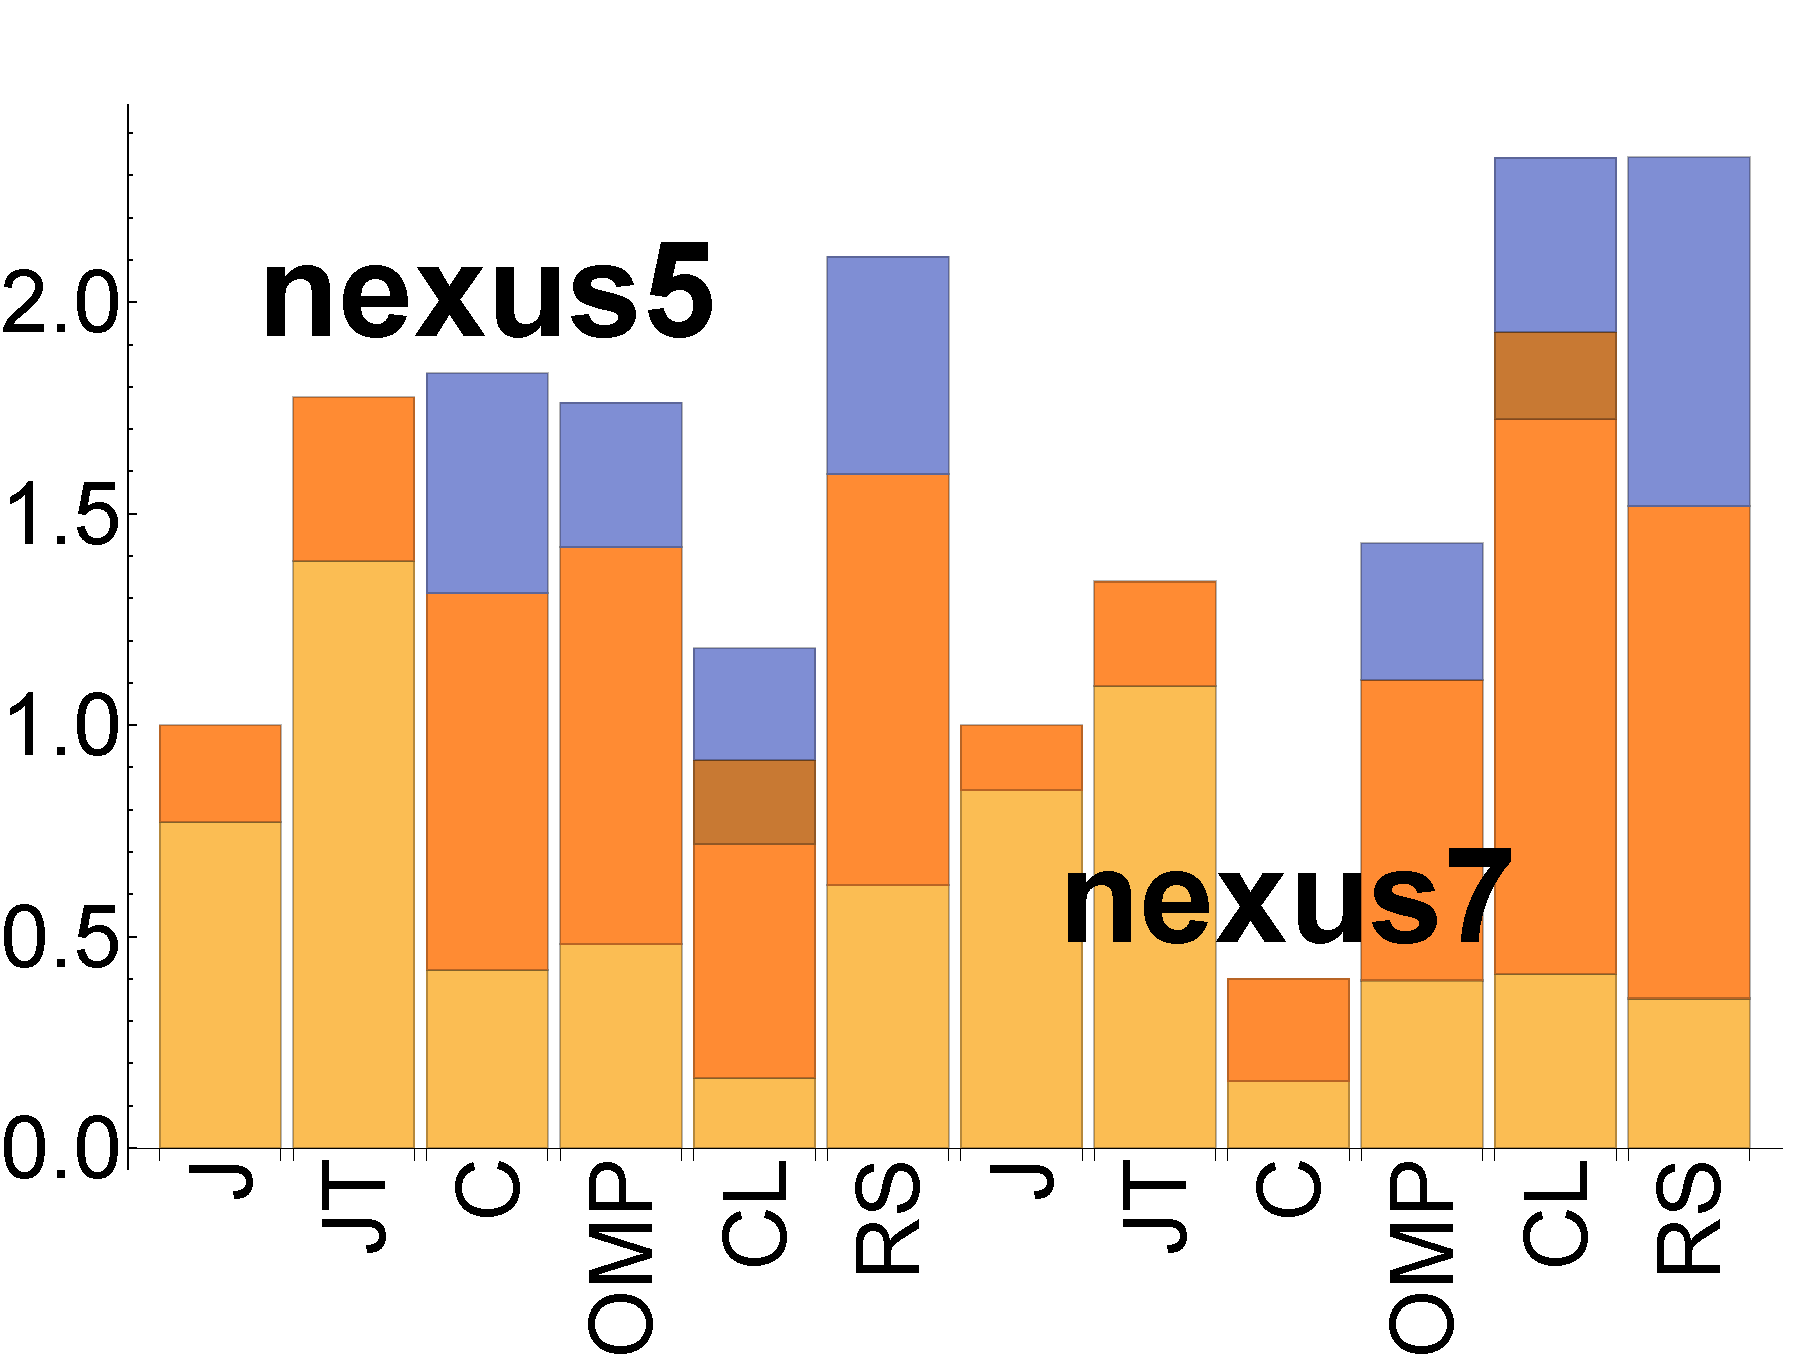
\includegraphics[width=\textwidth]{data/bbattery_vectoradd.pdf}
      \caption{VectorAdd}\label{fig:b_vectoradd}
  \end{subfigure}%

  \begin{subfigure}[b]{0.24\textwidth}
      \centering
      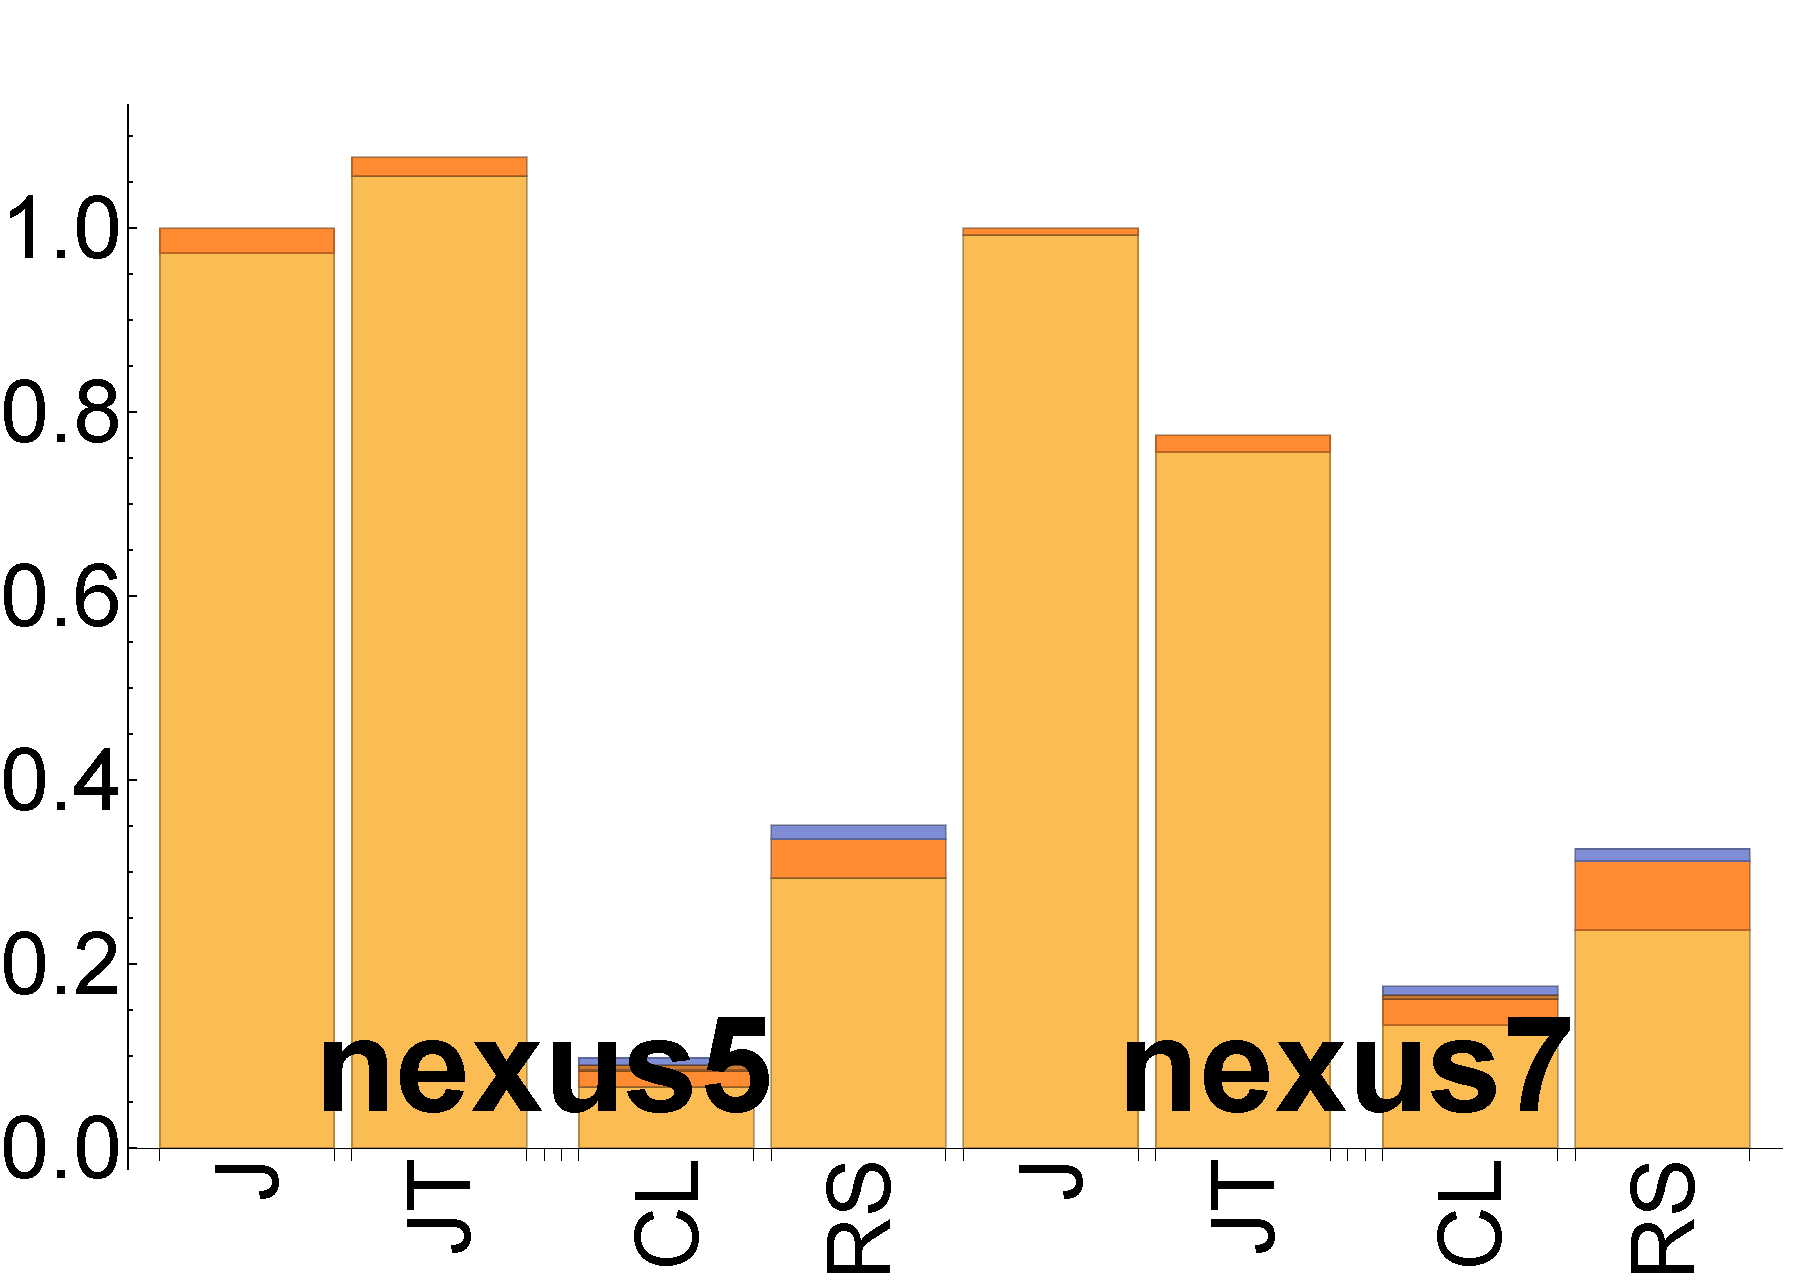
\includegraphics[width=\textwidth]{data/bbattery_tpacf.pdf}
      \caption{TPACF} \label{fig:b_TPACF}
  \end{subfigure}%

  \begin{subfigure}[b]{0.24\textwidth}
      \centering
      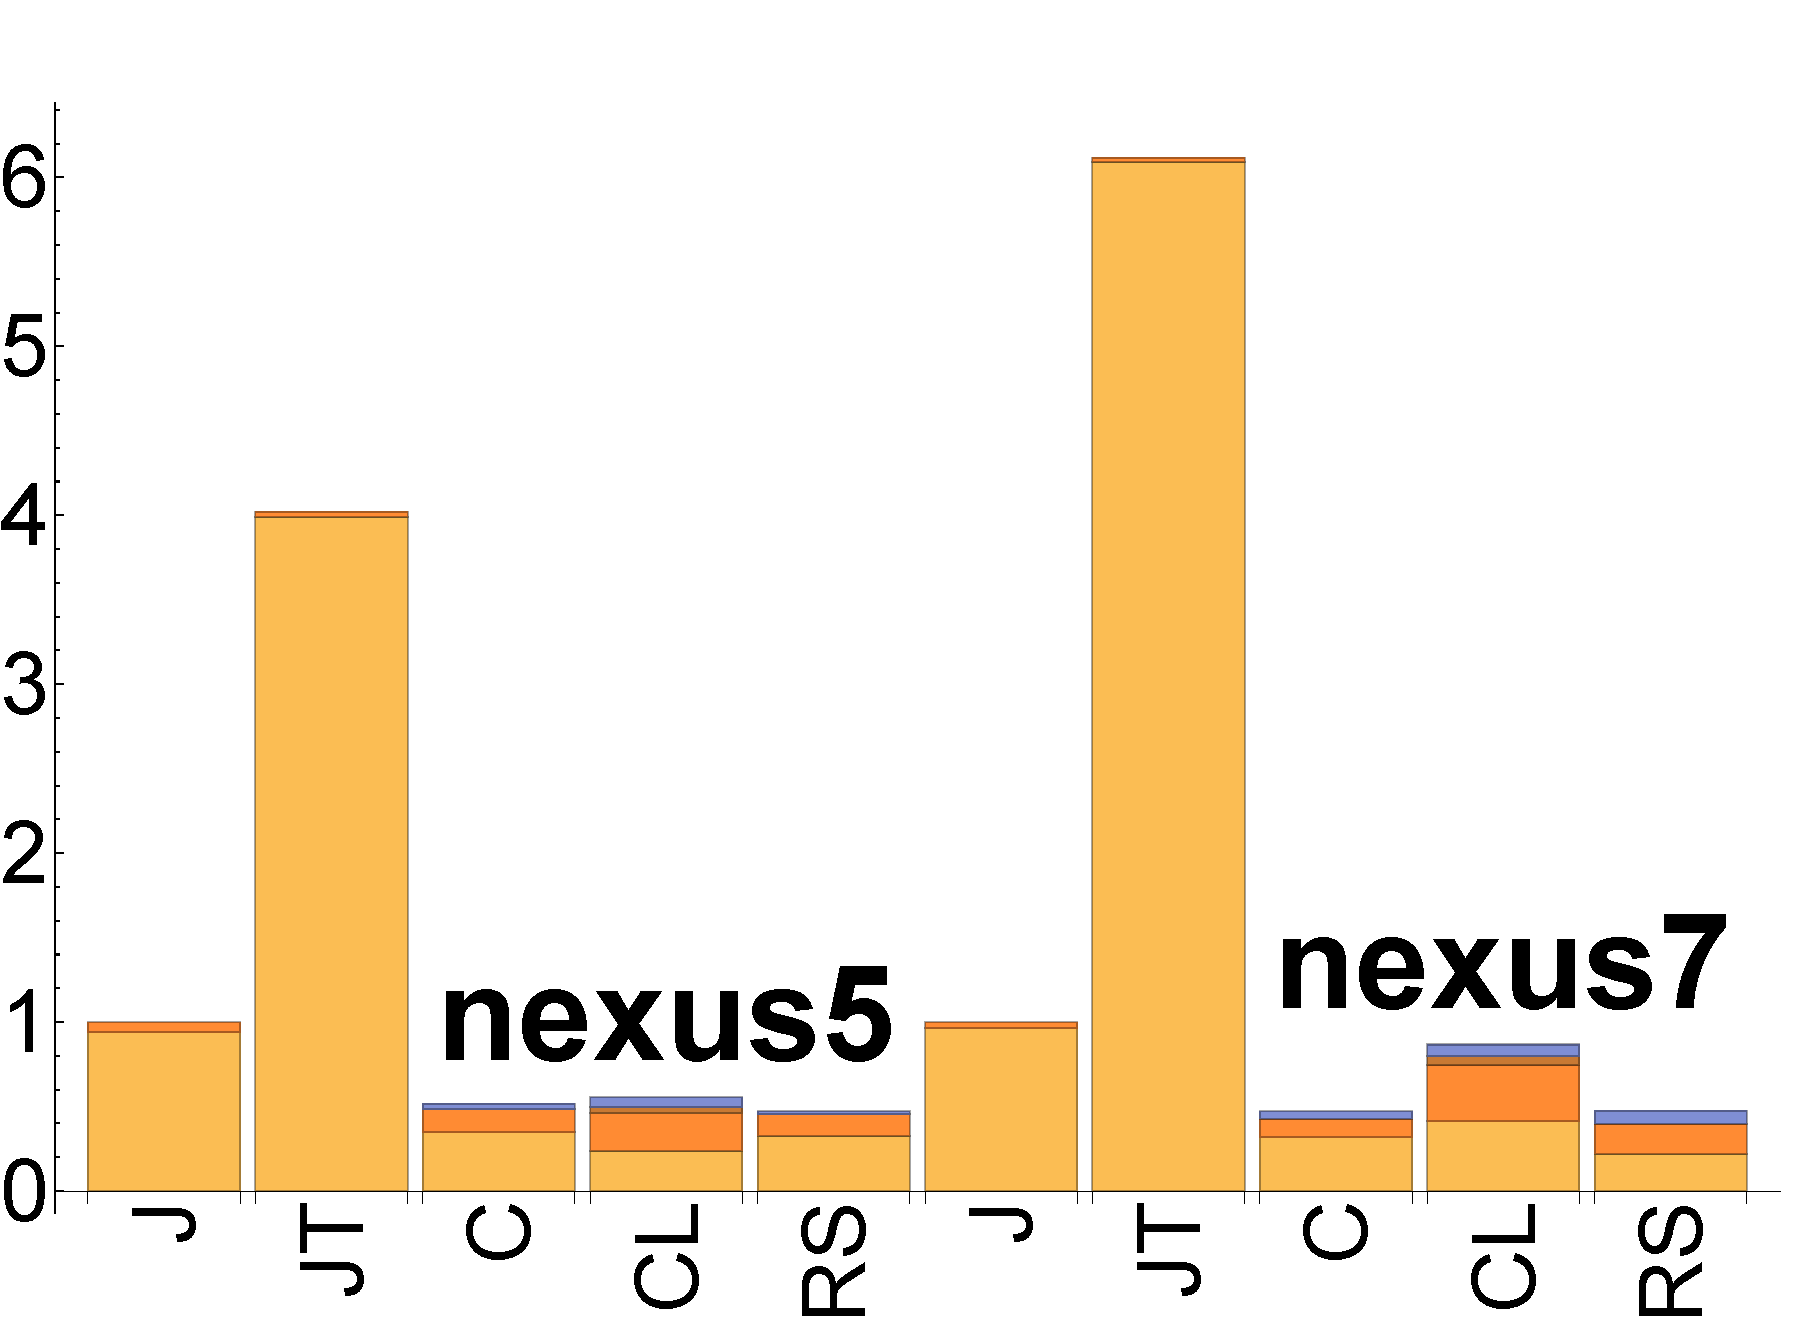
\includegraphics[width=\textwidth]{data/bbattery_histogram.pdf}
      \caption{Histo}\label{fig:b_histo}
  \end{subfigure}%

  \begin{subfigure}[b]{0.24\textwidth}
      \centering
      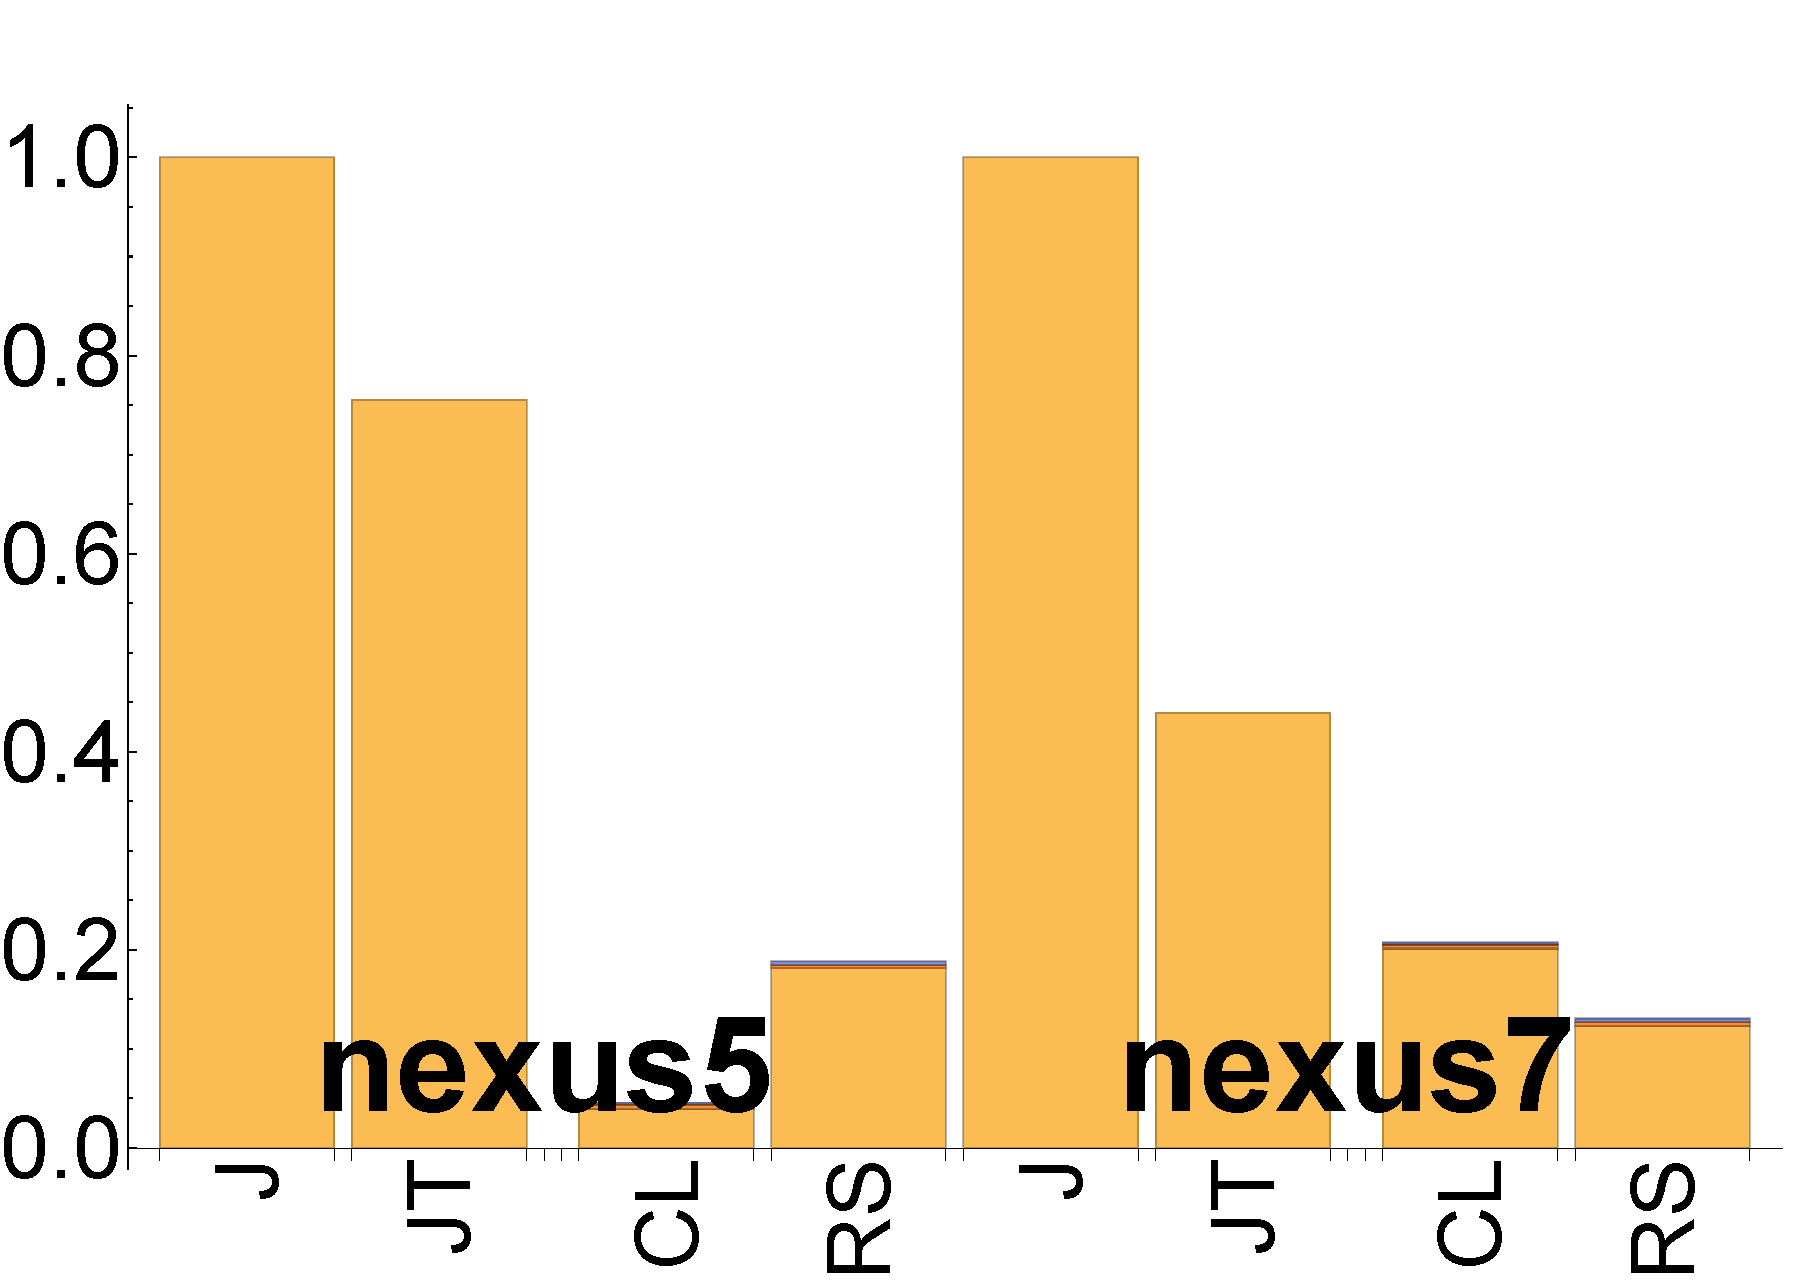
\includegraphics[width=\textwidth]{data/bbattery_mriq.pdf}
      \caption{MRIQ} \label{fig:b_MRIQ}
  \end{subfigure}

  \begin{subfigure}[b]{0.24\textwidth}
      \centering
      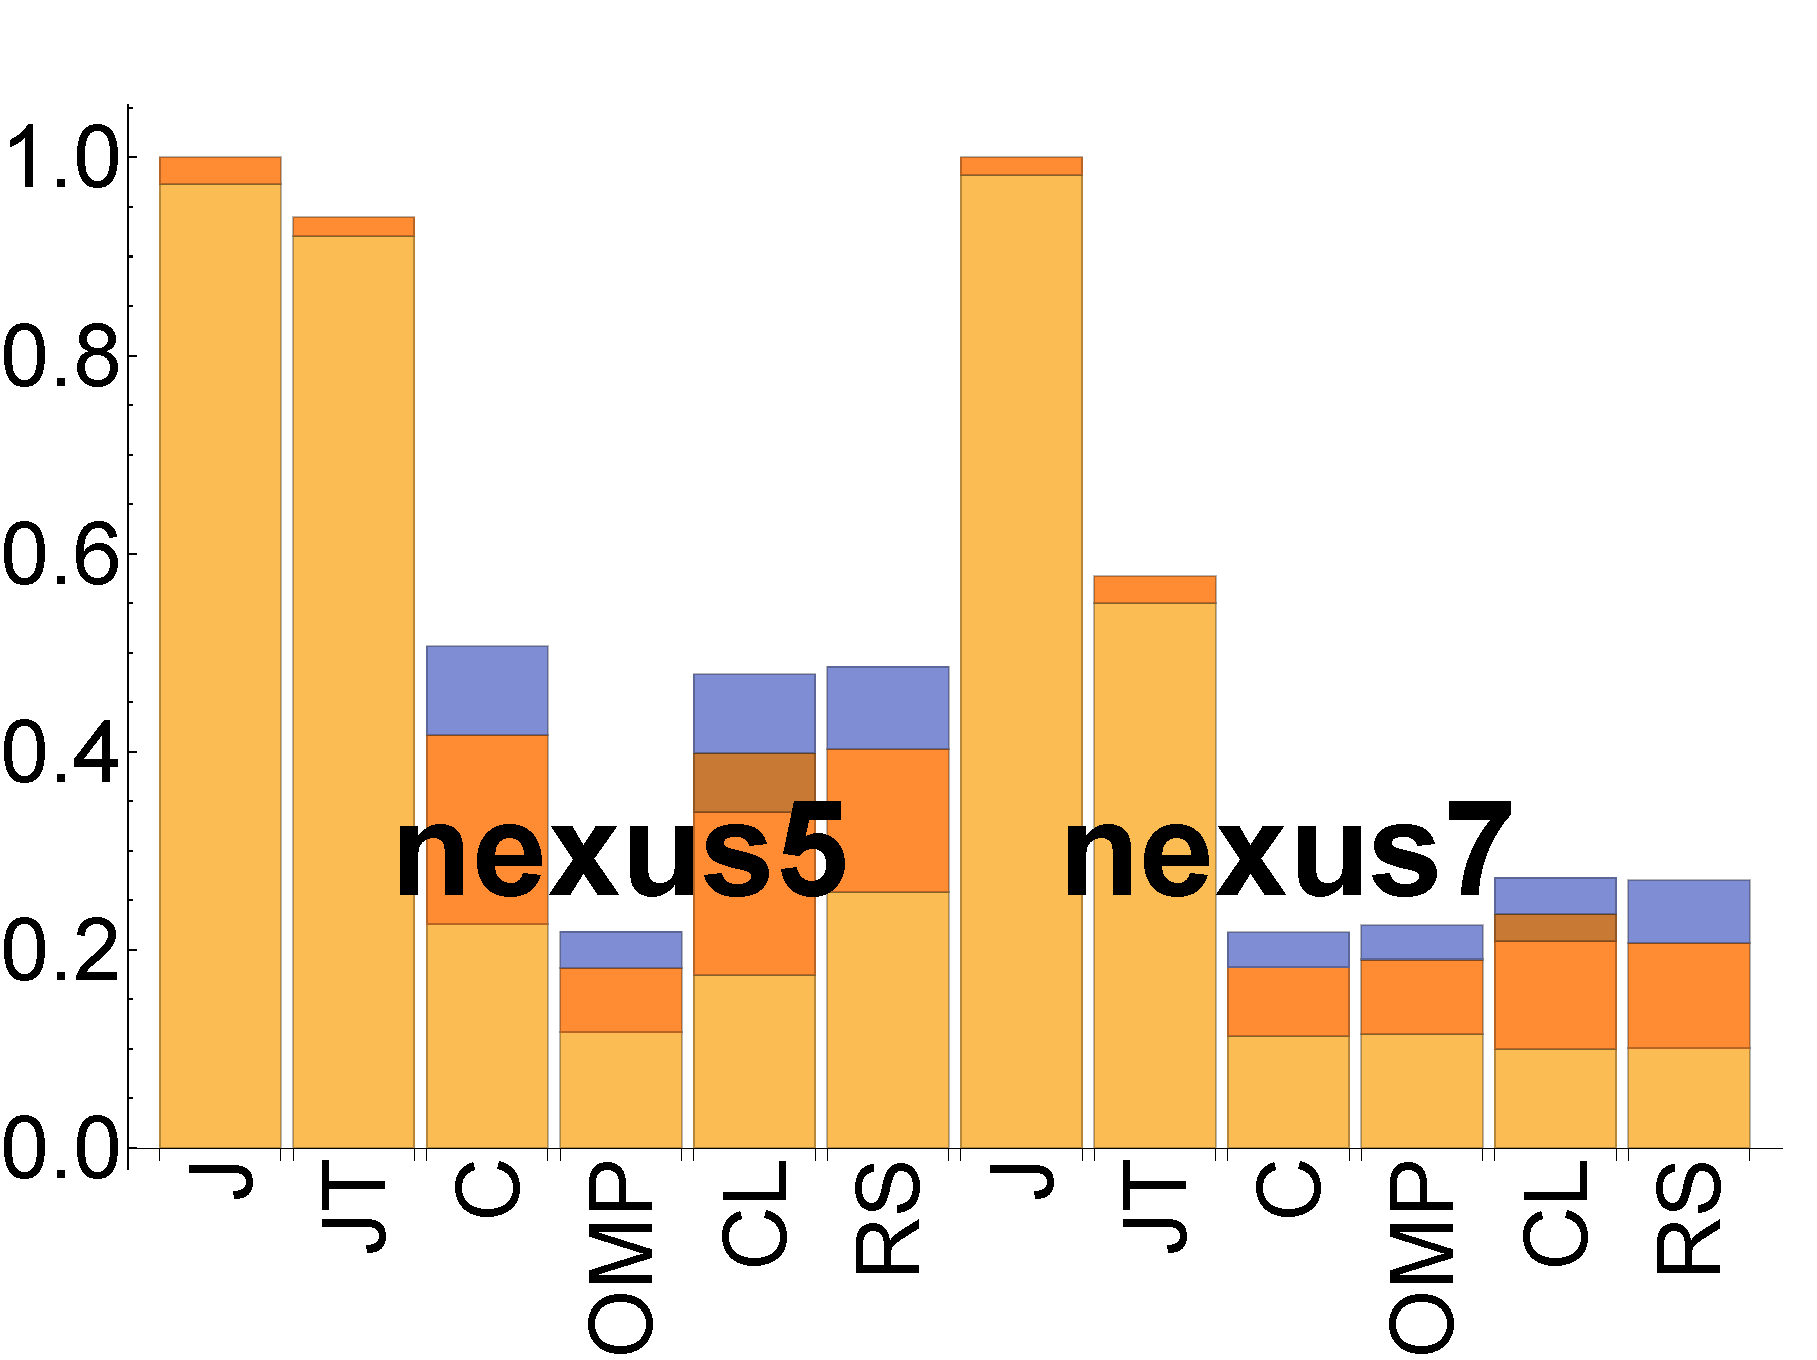
\includegraphics[width=\textwidth]{data/bbattery_sgemm.pdf}
      \caption{Sgemm}\label{fig:b_Sgemm}
  \end{subfigure}

  \begin{subfigure}[b]{0.24\textwidth}
      \centering
      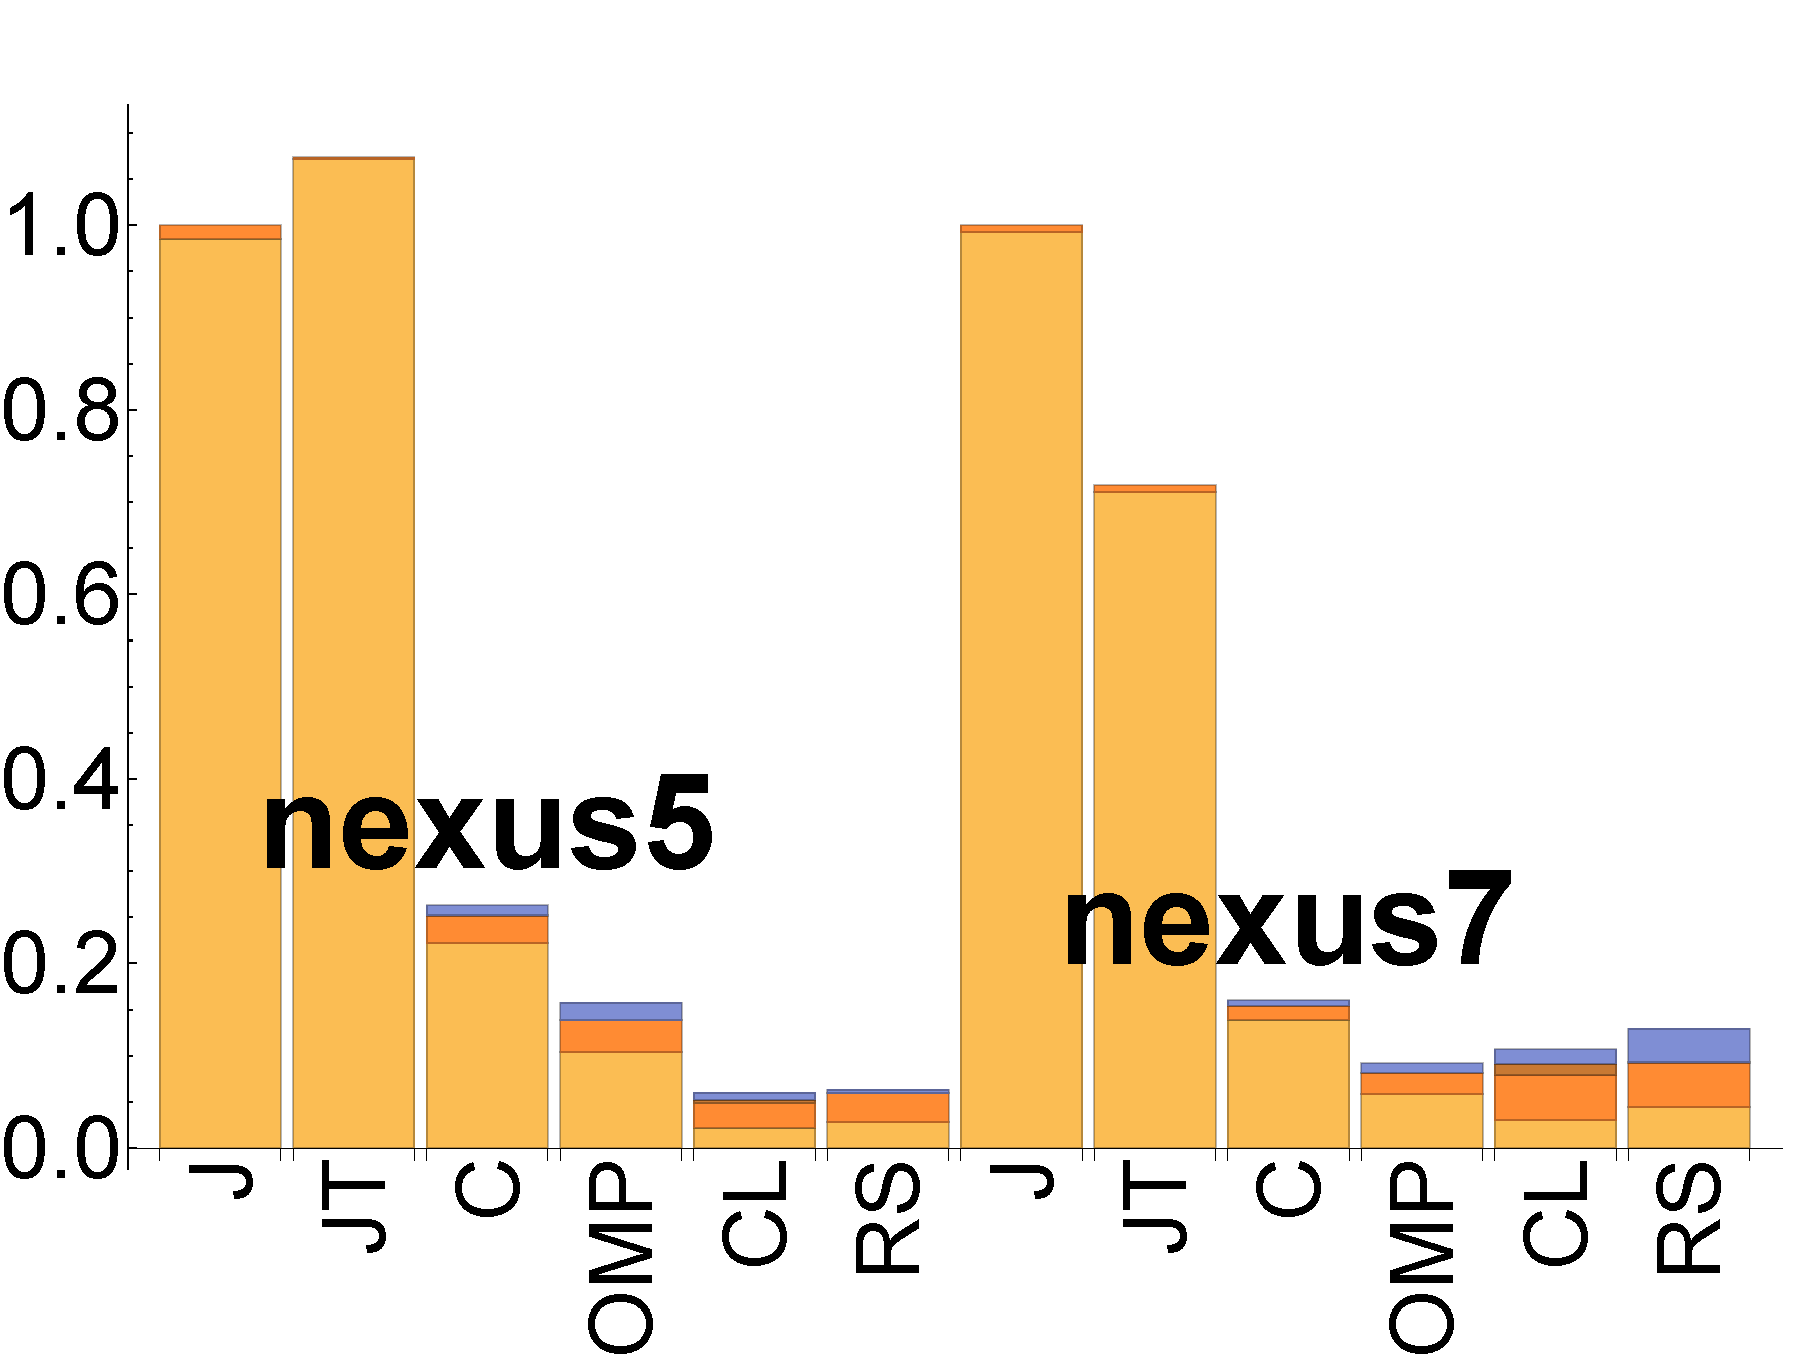
\includegraphics[width=\textwidth]{data/bbattery_stencil.pdf}
      \caption{Stencil} \label{fig:b_Stencil}
  \end{subfigure}

  \caption{Battery Information}
\end{figure}
\FloatBarrier



\subsubsection{Vector Add}

\subsubsection{SGEMM}

\subsubsection{Stencil}

\subsubsection{TPACF}

\subsubsection{MriQ}

\subsubsection{Histogram}

\subsubsection{CUTCP}

\subsection{Input/Output}

Throughout the analysis, we have ignored IO times which is in fact the biggest performance bottleneck in these benchmarks.
The main bottle neck is read speeds, since unlike desktops which have a hard drive read speed of 80-100MB/s, mobile devices typically use use flash which have a 7-25MB/s read speed.
In reality, however, computational data for mobile devices are not stored on disk and are usually either streamed from the cloud or captured from onboard sensors and therefore are available in RAM.
To keep with the typical usage, and to not skew the plots, we therefore explicitly removed the IO performance times from our graphs.


\subsection{RenderScript Programmability}
This section presents our analysis of RenderScript's programmability --- how
comfortable we, as programmers, feel when working with RenderScript. Since this
analysis is primarily based on our experience working with RenderScript
throughout this semester, it is highly subjective. Additionally, we are aware
that some of the limitations presented in this section are due to the fact that
RenderScript is a new framework, which is being rapidly developed and deployed.
Therefore, we expect that RenderScript will keep evolving to close many of the
identified limitations.

\paragraph{The Goods.}
We start by describing the features that we like about the RenderScript.

\textit{RenderScript delivers on its promises about code portability}.
The runtime behavior of our RenderScript implementations is consistent across
five different tested devices and seven different benchmarks. For example, we
always got the same runtime errors, e.g., segmentation fault or out-of-memory
error, regardless of the devices that the code is running on. Furthermore, we
did not have to express any device specific parameters in our code. The code
portability gives us a confidence that if a kernel works on our testing device,
it will work seamlessly on other devices. OpenCL, on the other hand, required
tuning some
parameters, such as work-group sizes, in order to avoid crashes when ported to
other devices.

\subsubsection{Debug Support}

Since RenderScript is natively supported in Android,
it offers a set of convenient built-in debugging
facilities, such as the \fix{rsDebug()} functions, detailed runtime exceptions,
and IDE-navigable compilation errors.
The \fix{rsDebug()} function forces RenderScript to execute on the CPU and interacts 
with the eclipse platform to offer a convinent way to present printed values from within the kernel
(OpenCL and CUDA offer similar facilities, but they are less convinent to use).
For programmers accustomed to \fix{printf()} debugging style in C/C++, this interface provides
a familiar debugging model. For developers expecting a breakpoint debugging workflow, the eclipse
environment has no facilities for that currently.


\subsubsection{Memory Operations}

The \fix{Allocation} interface is intuitive to express data and
execution parallelism}. As described in section~\ref{sec:imple_RS}, this
\fix{Allocation} interface allows explicitly expressing parallelism
granularities, i.e., via packing output and/or input into \fix{Element} objects,
for RenderScript kernels.  We quickly got used to this interface
after completing the first set of simple benchmarks, and we did not encounter
any problems using this interface.

Within the kernel, utility functions (\fix{rsGetElementAt_*}) make indexing
 into a multi-dimensional arrays platform agnostic
 (e.g. the strides should not be assumed to be the same across architectures).


\subsubsection{Familiar Language}

\textit{Writing RenderScript kernel in C99 brings great flexibility and
performability\todo{Is this a word? What do you mean by performability}}. We
liked the feeling of having complete control when using
the C language for performance critical code. We understand that this point is
completely biased due to our proficiency with C, C++, and CUDA. For many
programmers, it is an abrupt transition from programming in Java to programming
in C.

\paragraph{The Bads.} We also found that RenderScript was still unpleasant to
work with as it has some unnecessary idiosyncratic restrictions. However, many
of these limitations exist due to the
infancy of the framework.

\subsubsection{Lack of Intrinsics}

\textit{No intrinsic synchronization within kernels.} Currently, RenderScript
only allows global synchronization by calling the \fix{syncAll()} function in
Java host code. This means that there is no CUDA-like \fix{\_\_syncthread()} or
OpenCL-like \fix{barrier()} functions that can be called inside RenderScript
kernels. Therefore, RenderScript kernels do not allow threads to share
intermediate data. We found that this model is too restrictive in several
scenarios. For example in the \fix{CUTCP} benchmark, we had to substantially
modify the RenderScript \todo{Do you mean OpenCL implementation} implementation in order
to overcome the lack of
synchronization support.

\subsubsection{Multi-Dimensional Parallelism}


\textit{Lack of support for multi-dimensional parallelism}. A RenderScript
kernel allows an \fix{Allocation} to specify \fix{X}, \fix{Y}, and \fix{Z}
dimensions, and the workload would be distributed across hardware units using
these dimensions. However, currently it only supports two
dimensions. The interface for the third dimension exists but was not
implemented.

\subsubsection{Non-Unified Memory}

Before RenderScript execution starts, all
heap data to be used by the kernel has to copied into \fix{Allocation} buffers.
The buffer has to be copied back to make it available to Java.
Safe casting between Java and C requires some checking --- since Java does not 
  conform to the same IEEE standard that RenderScript conforms to.
But in the case of unsafe copies, these can be avoided when the kernel is
  executing in the same coherence domain.
The current implementation of RenderScript does not perform these optimizations.
Furthermore, the runtime, via function overloading, should be able to hide 
  explicit buffer creation and copies, by detecting the type passed into the function
  and converting to a \fix{Allocation} buffer if what is passed is a Java array.

\subsubsection{Lack of a Standardization}

RenderScript is similar to CUDA in this respect --- the reference implementation
  is the standard.
Yet unlike CUDA, RenderScript's documentation tend to be incomplete and insufficient.
Atomic instructions such as \fix{rsAtomicInc(<Type>)}, for example, are claimed to be supported
in documentation and appear in the header files for several data types, but upon usage 
the runtime raises an exception if any type other than \fix{int32\_t} is used.
The lack of specification results in some errors being unintuitive --- one has to 
  read the runtime to determine what the error refers to and what caused it.
It also means that it is unlikely that RenderScript would be 
  ported to desktop platforms.


\subsubsection{Another Parallel Framework}

Aside from having full control over the language, it is not clear why
 Google did not adopt OpenCL or OpenCL's SPIR layer.
As can be seen, the RenderScript language borrows many elements from the CUDA/OpenCL 
 programming model, with some tooling support.
Many of the ``features'' of RenderScript can be implementing via a library that 
 interacts with OpenCL and there is no need for a new language.
One reason could be that the compiler and runtime can prevent compute code that run on the GPU from
 possibly crashing the driver (by using too much resources or using unsafe memory accesses),
 since crashing the GPU driver on mobile devices is equivalent to crashing the device.
Yet, again, this feature can be implemented by enhancing the OpenCL compiler and runtime to detect
 and raise an exception if illegal memory accesses occur.


